\documentclass{beamer}
\usetheme{default}

\usepackage{graphicx}
\usepackage{float}
\usepackage{tikz}

\title{Beamer Template}
\author{TeXstudio Team}
\begin{document}
\begin{frame}[plain]
    \maketitle
\end{frame}

\begin{frame}
	\begin{figure}
		\centering
		\resizebox{\textwidth}{!}{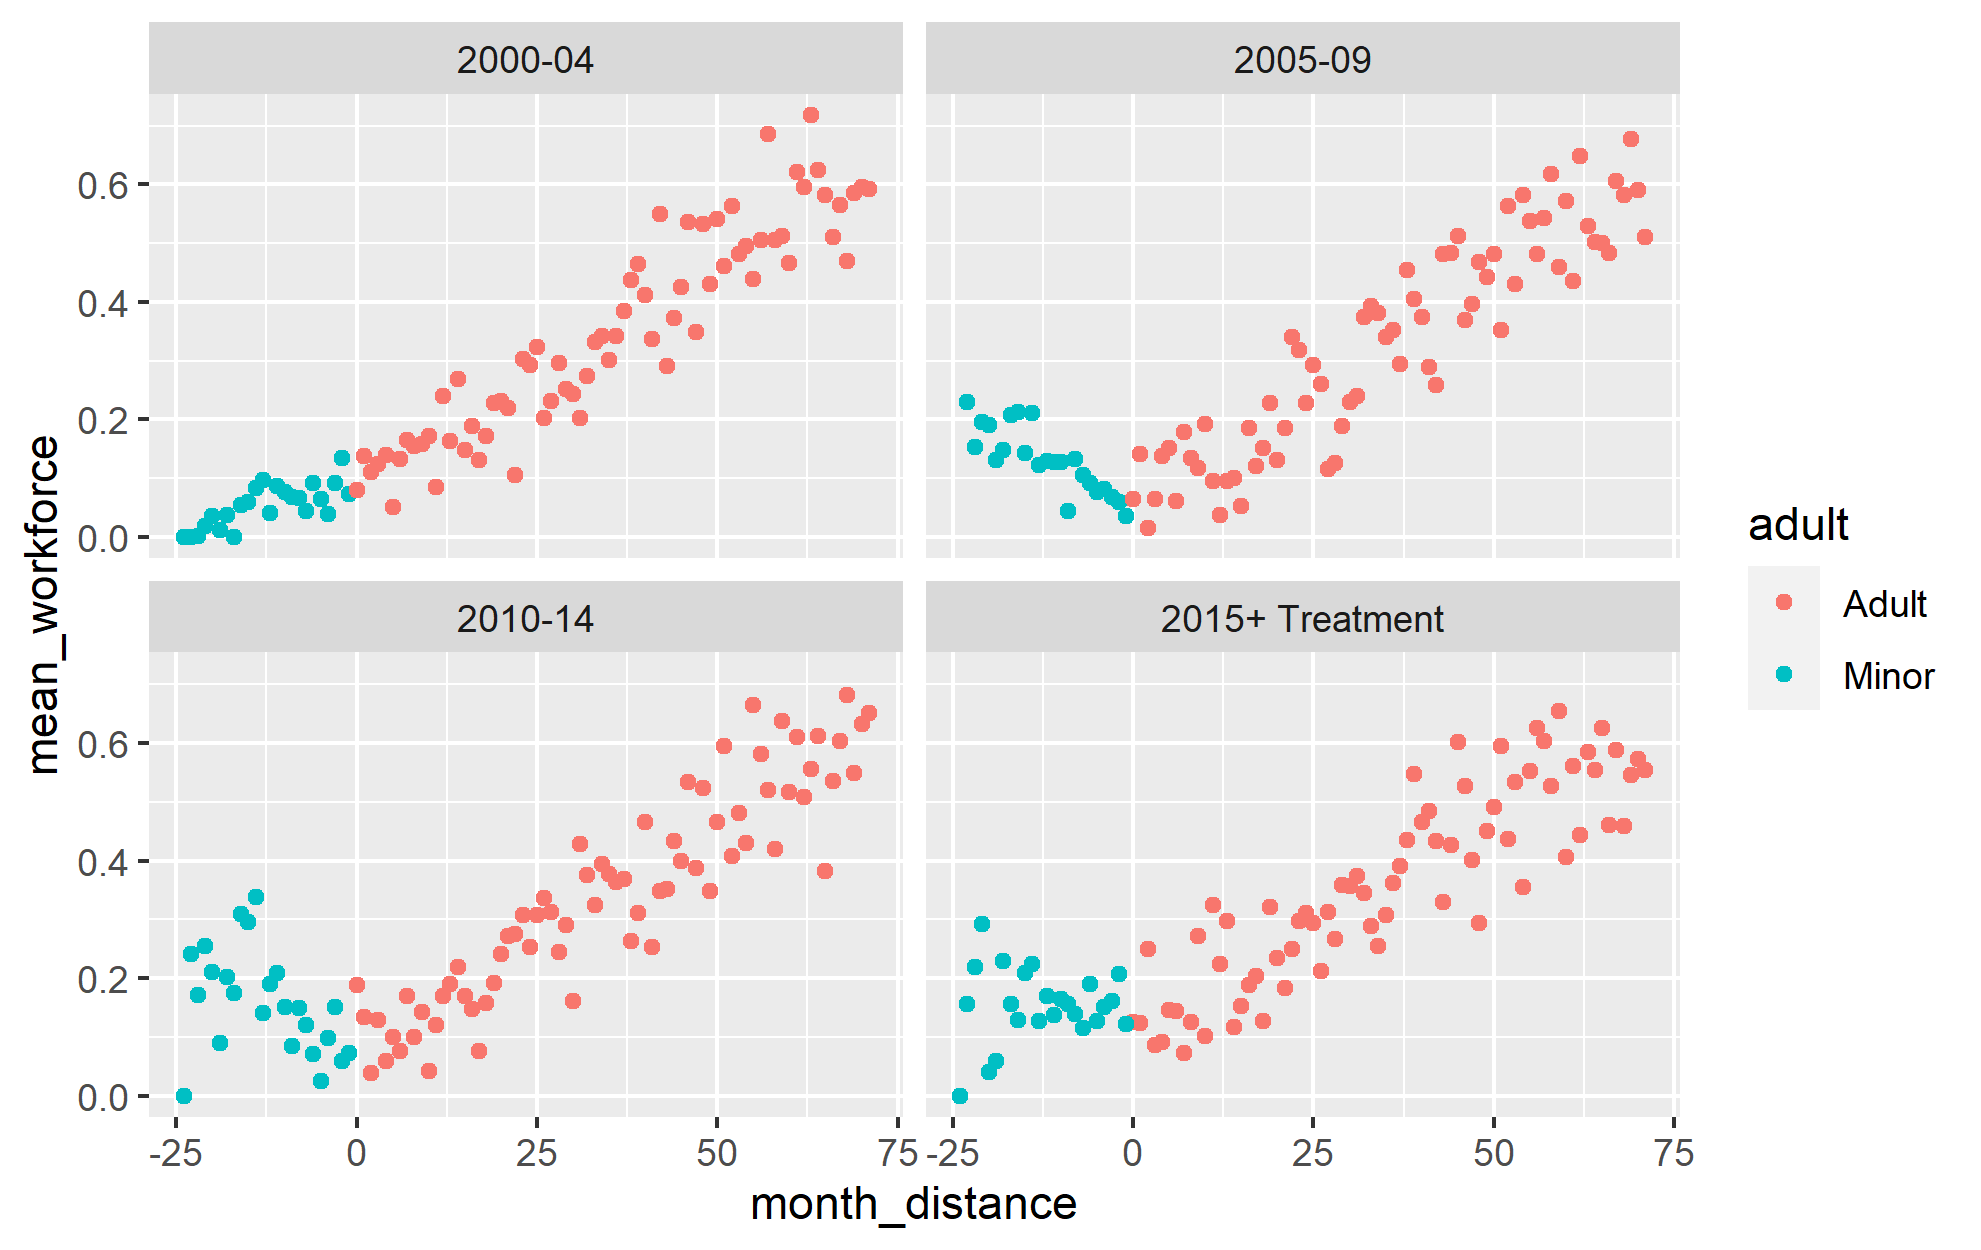
\includegraphics{../../plots/scatter_emp.png}}
	\end{figure}
\end{frame}

\begin{frame}
	\begin{figure}
		\centering
		\resizebox{\textwidth}{!}{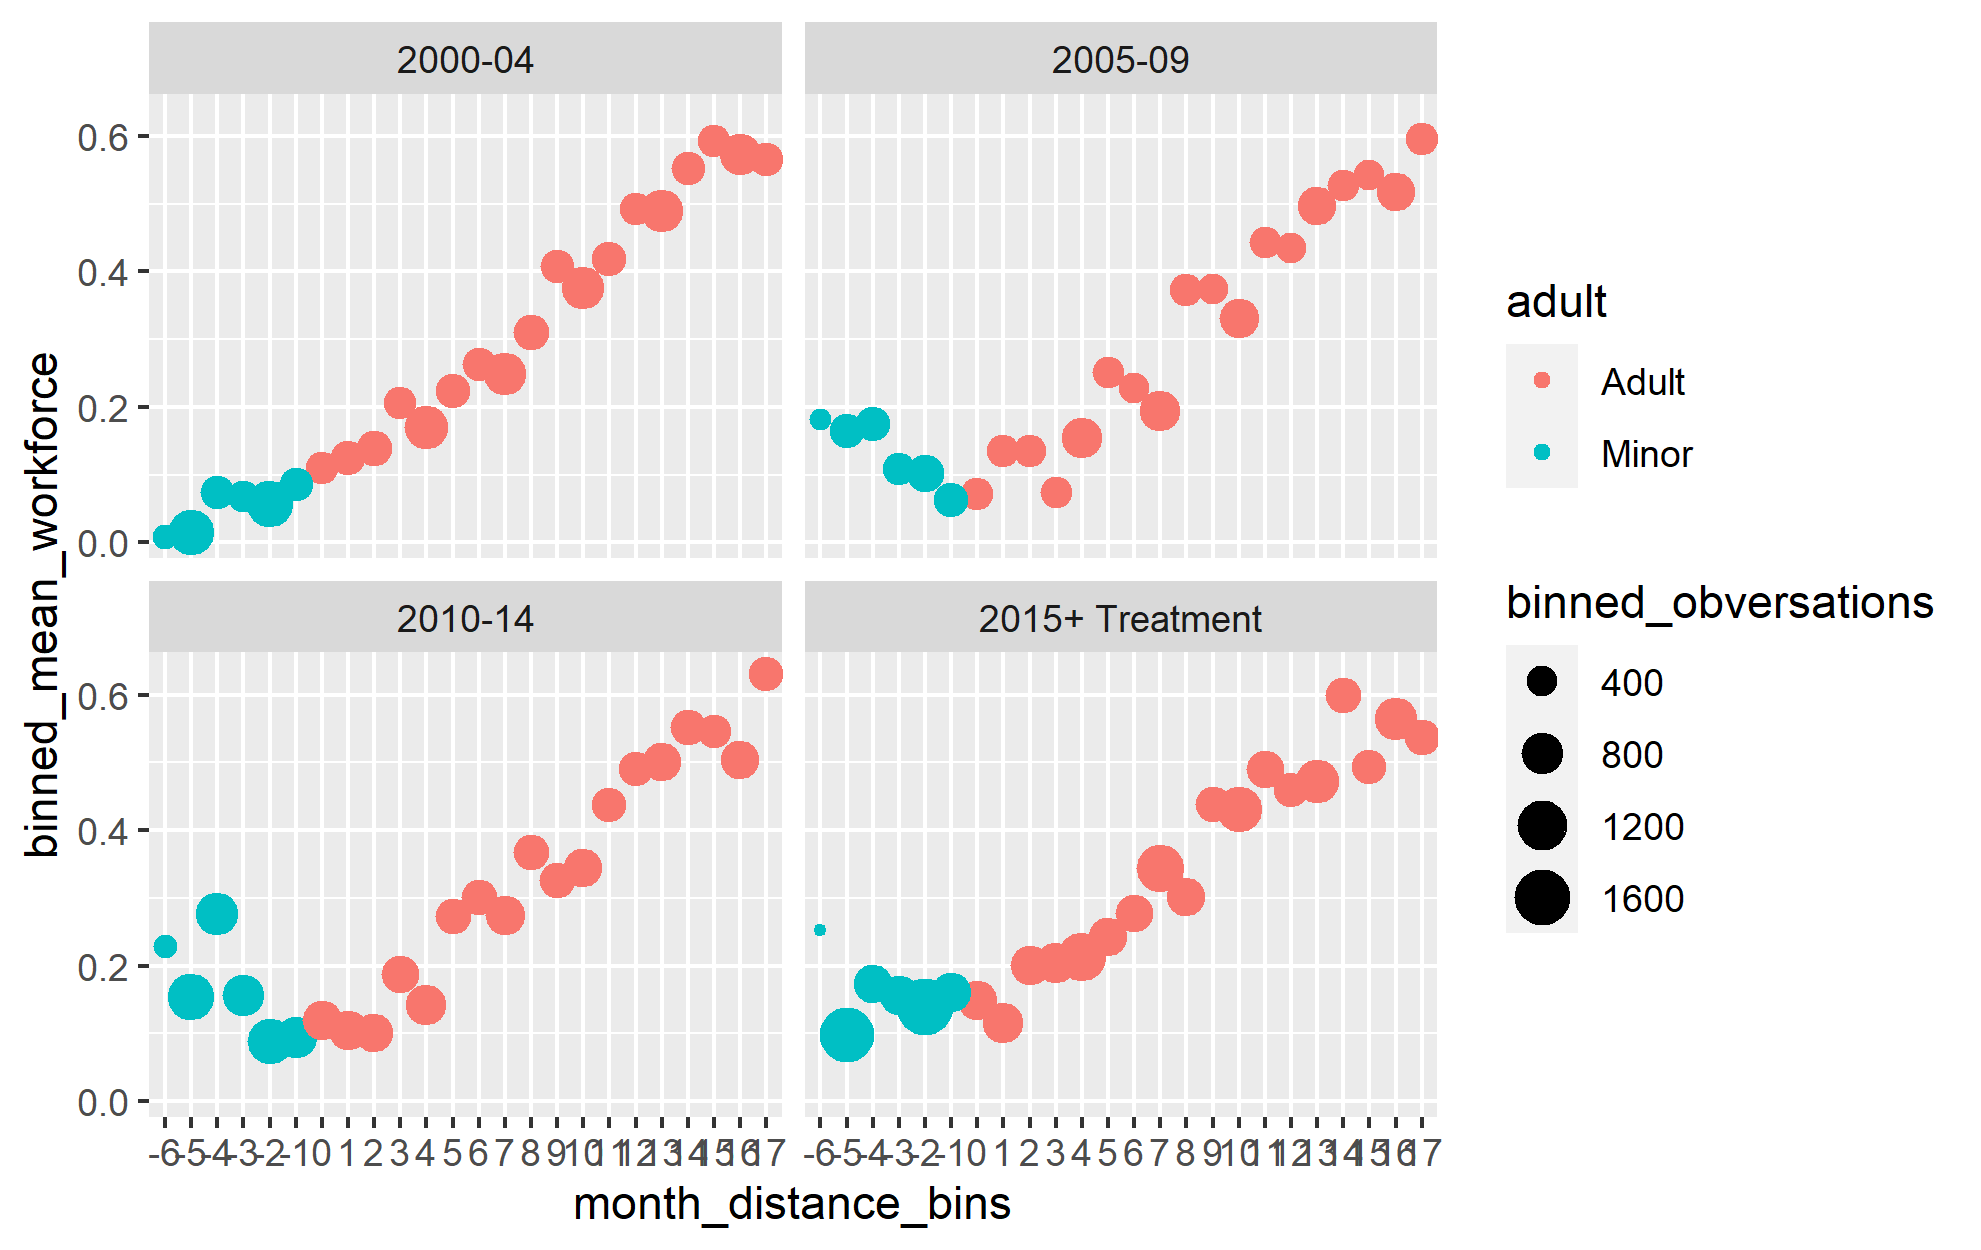
\includegraphics{../../plots/binned_emp_scatter.png}}
	\end{figure}
\end{frame}

\begin{frame}
	\begin{figure}
		\centering
		\resizebox{\textwidth}{!}{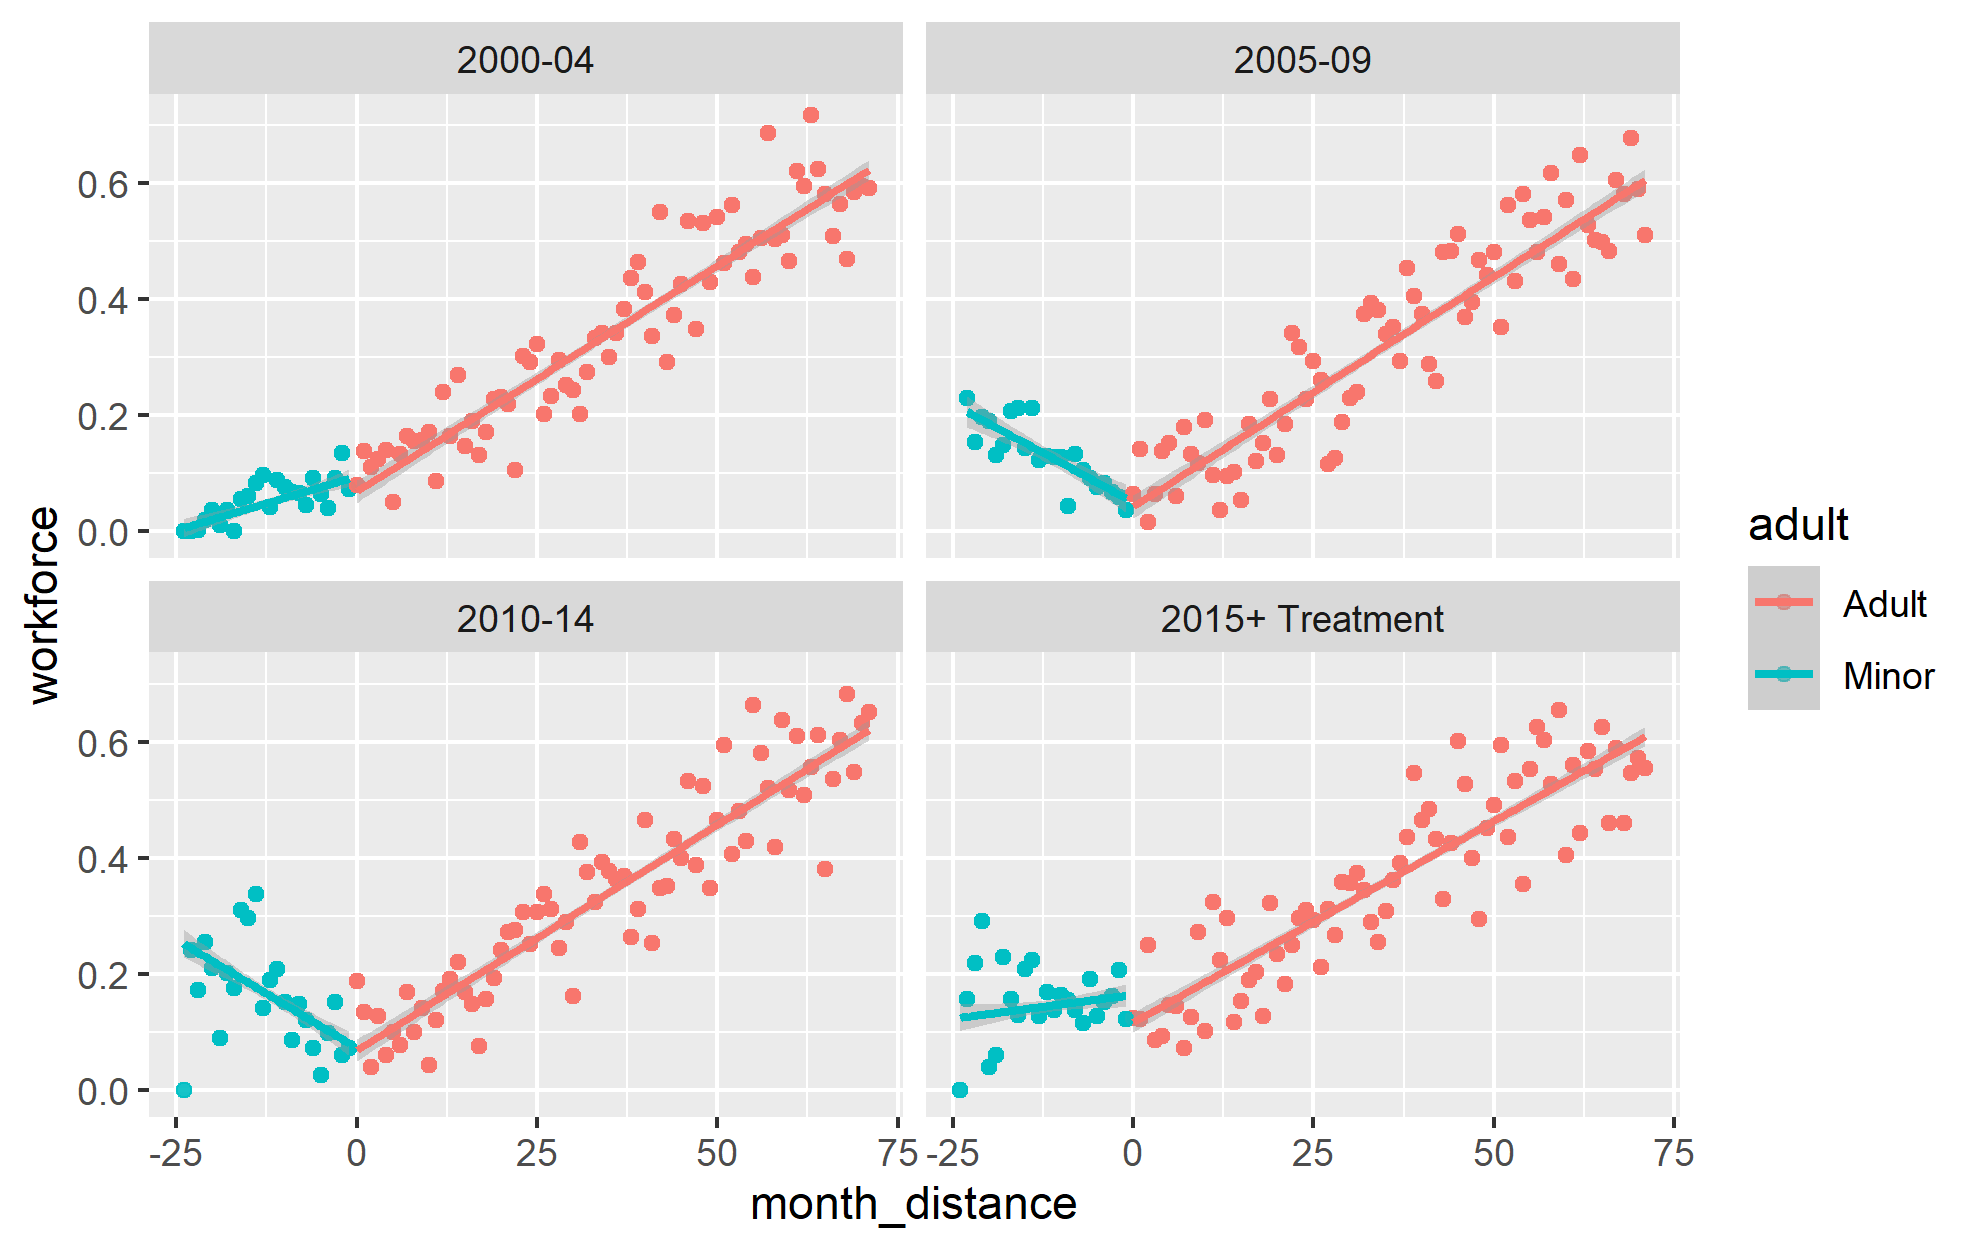
\includegraphics{../../plots/employment_linear.png}}
	\end{figure}
\end{frame}

\begin{frame}
	\begin{figure}
		\centering
		\resizebox{\textwidth}{!}{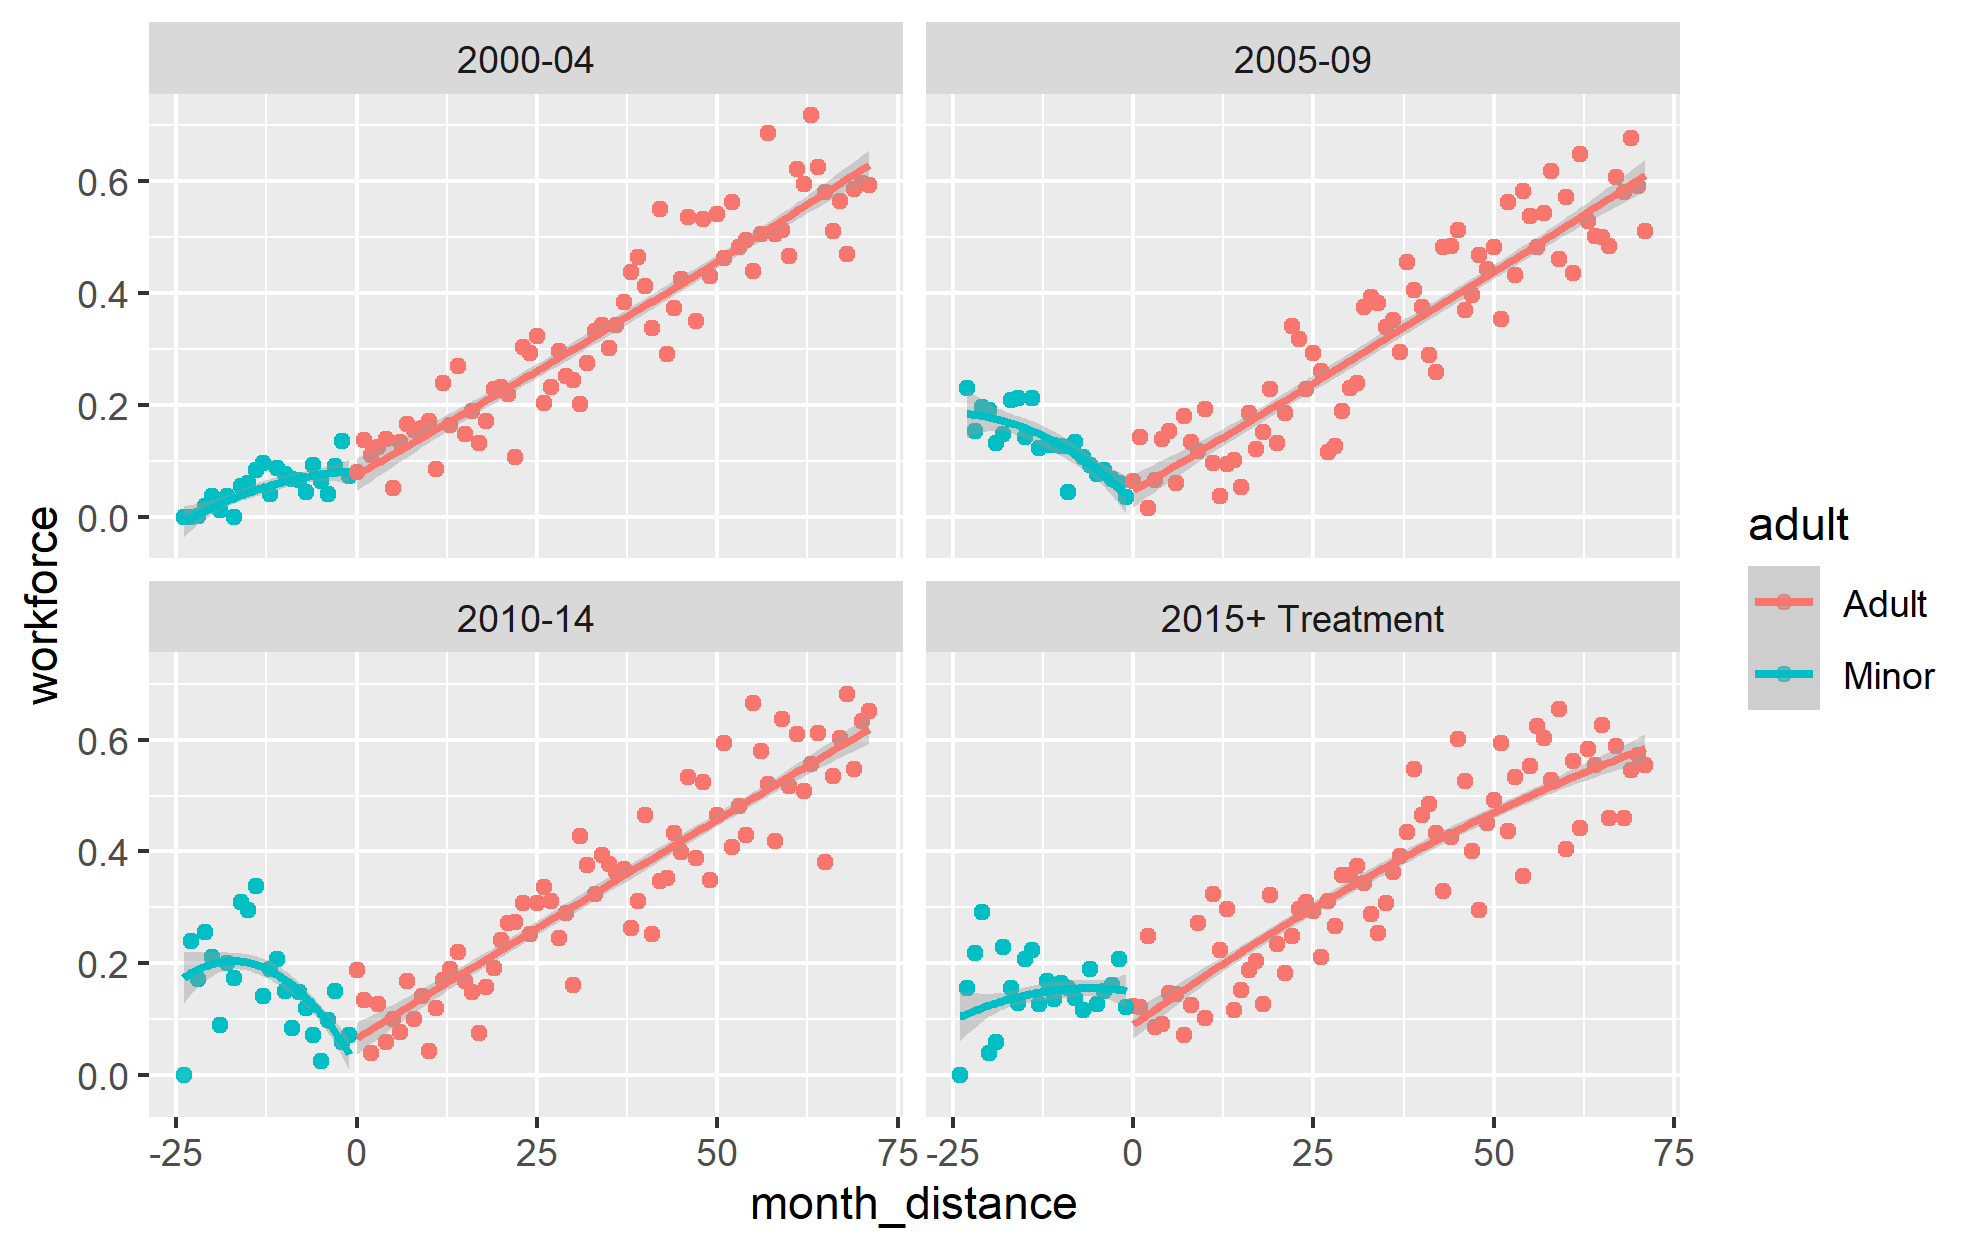
\includegraphics{../../plots/employment_quadratic.png}}
	\end{figure}
\end{frame}



\begin{frame}
	\begin{figure}
		\centering
		\resizebox{\textwidth}{!}{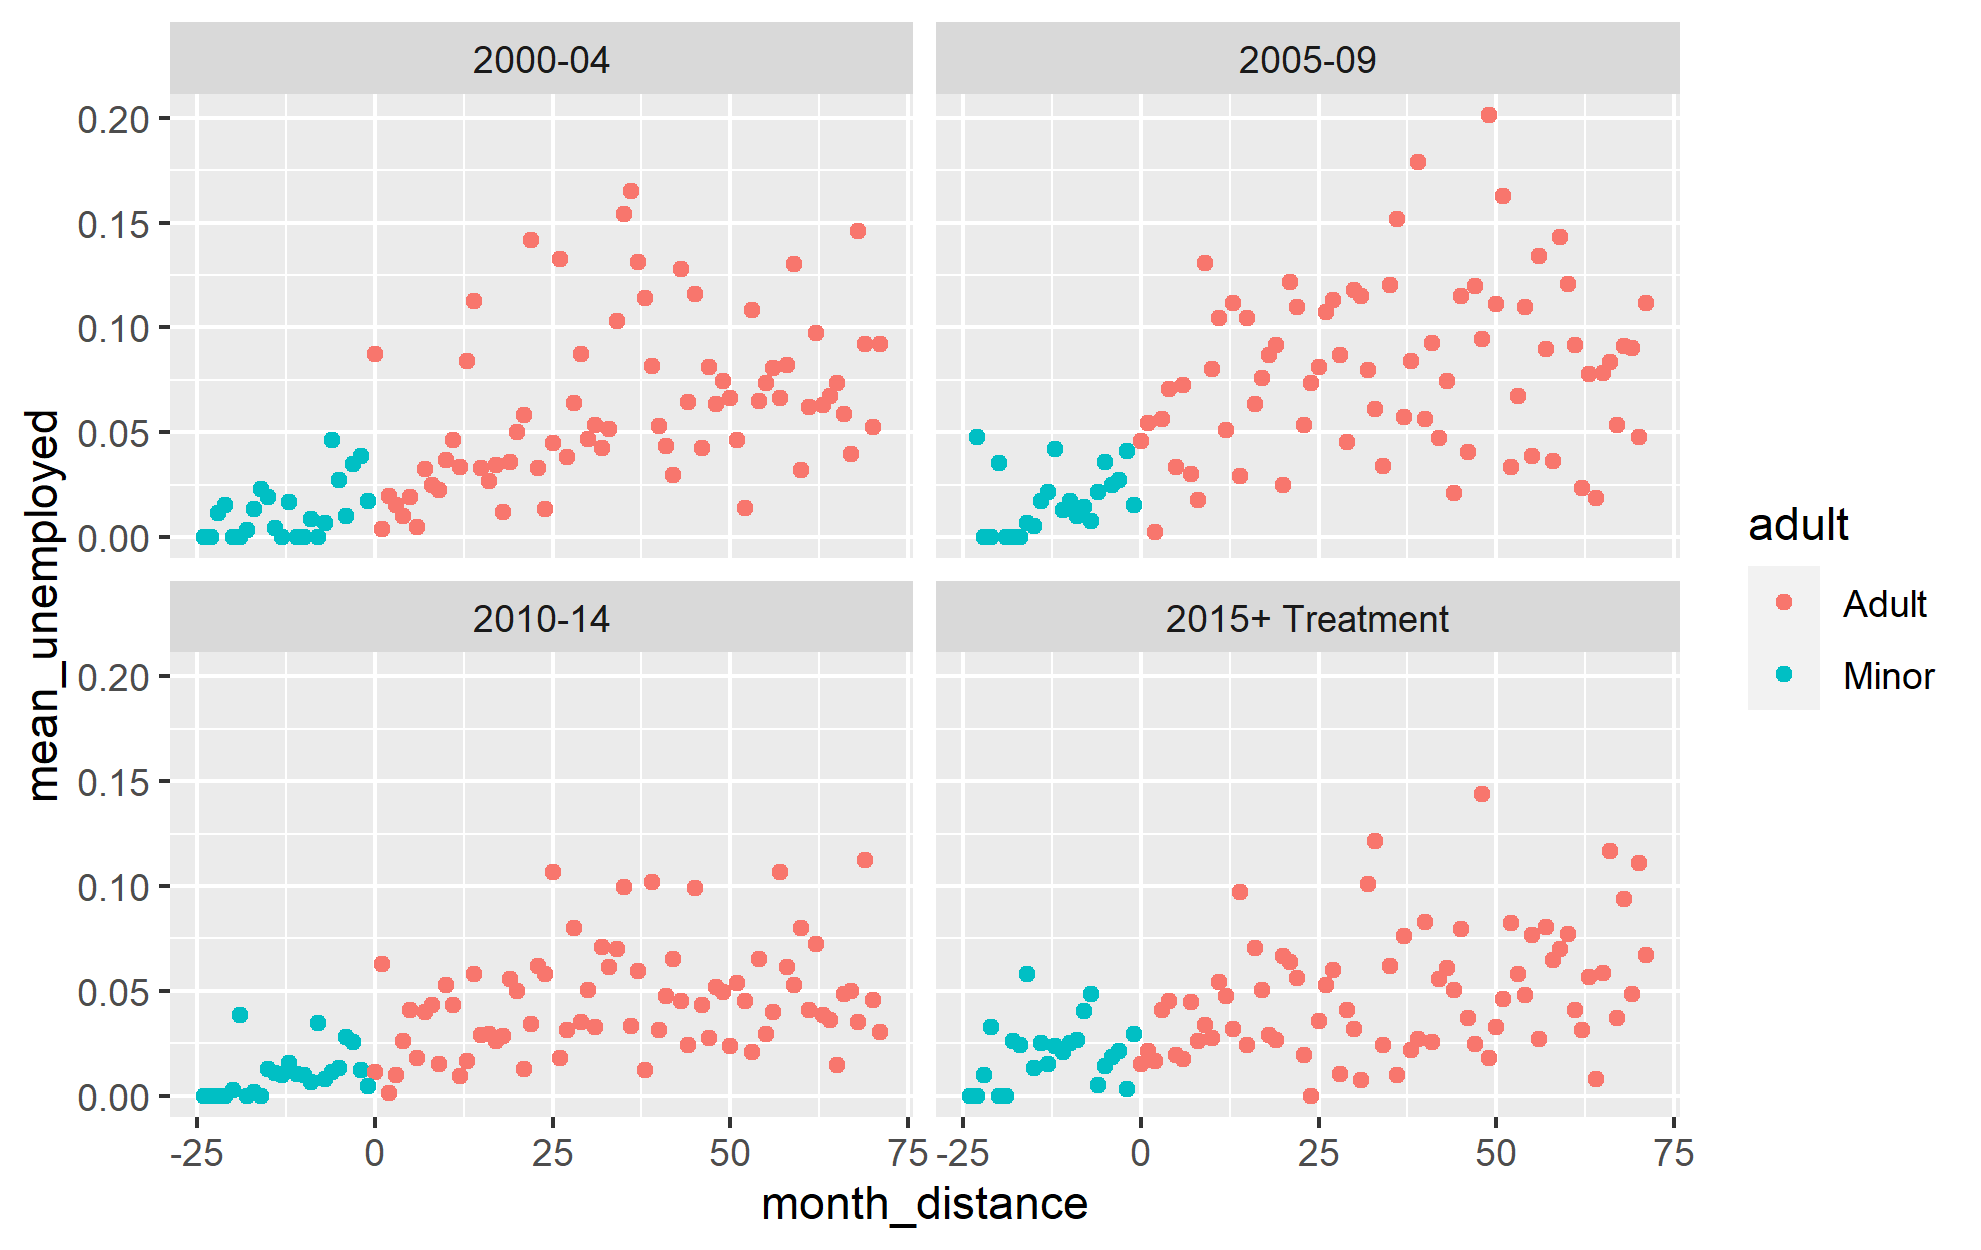
\includegraphics{../../plots/scatter_unemp.png}}
	\end{figure}
\end{frame}

\begin{frame}
	\begin{figure}
		\centering
		\resizebox{\textwidth}{!}{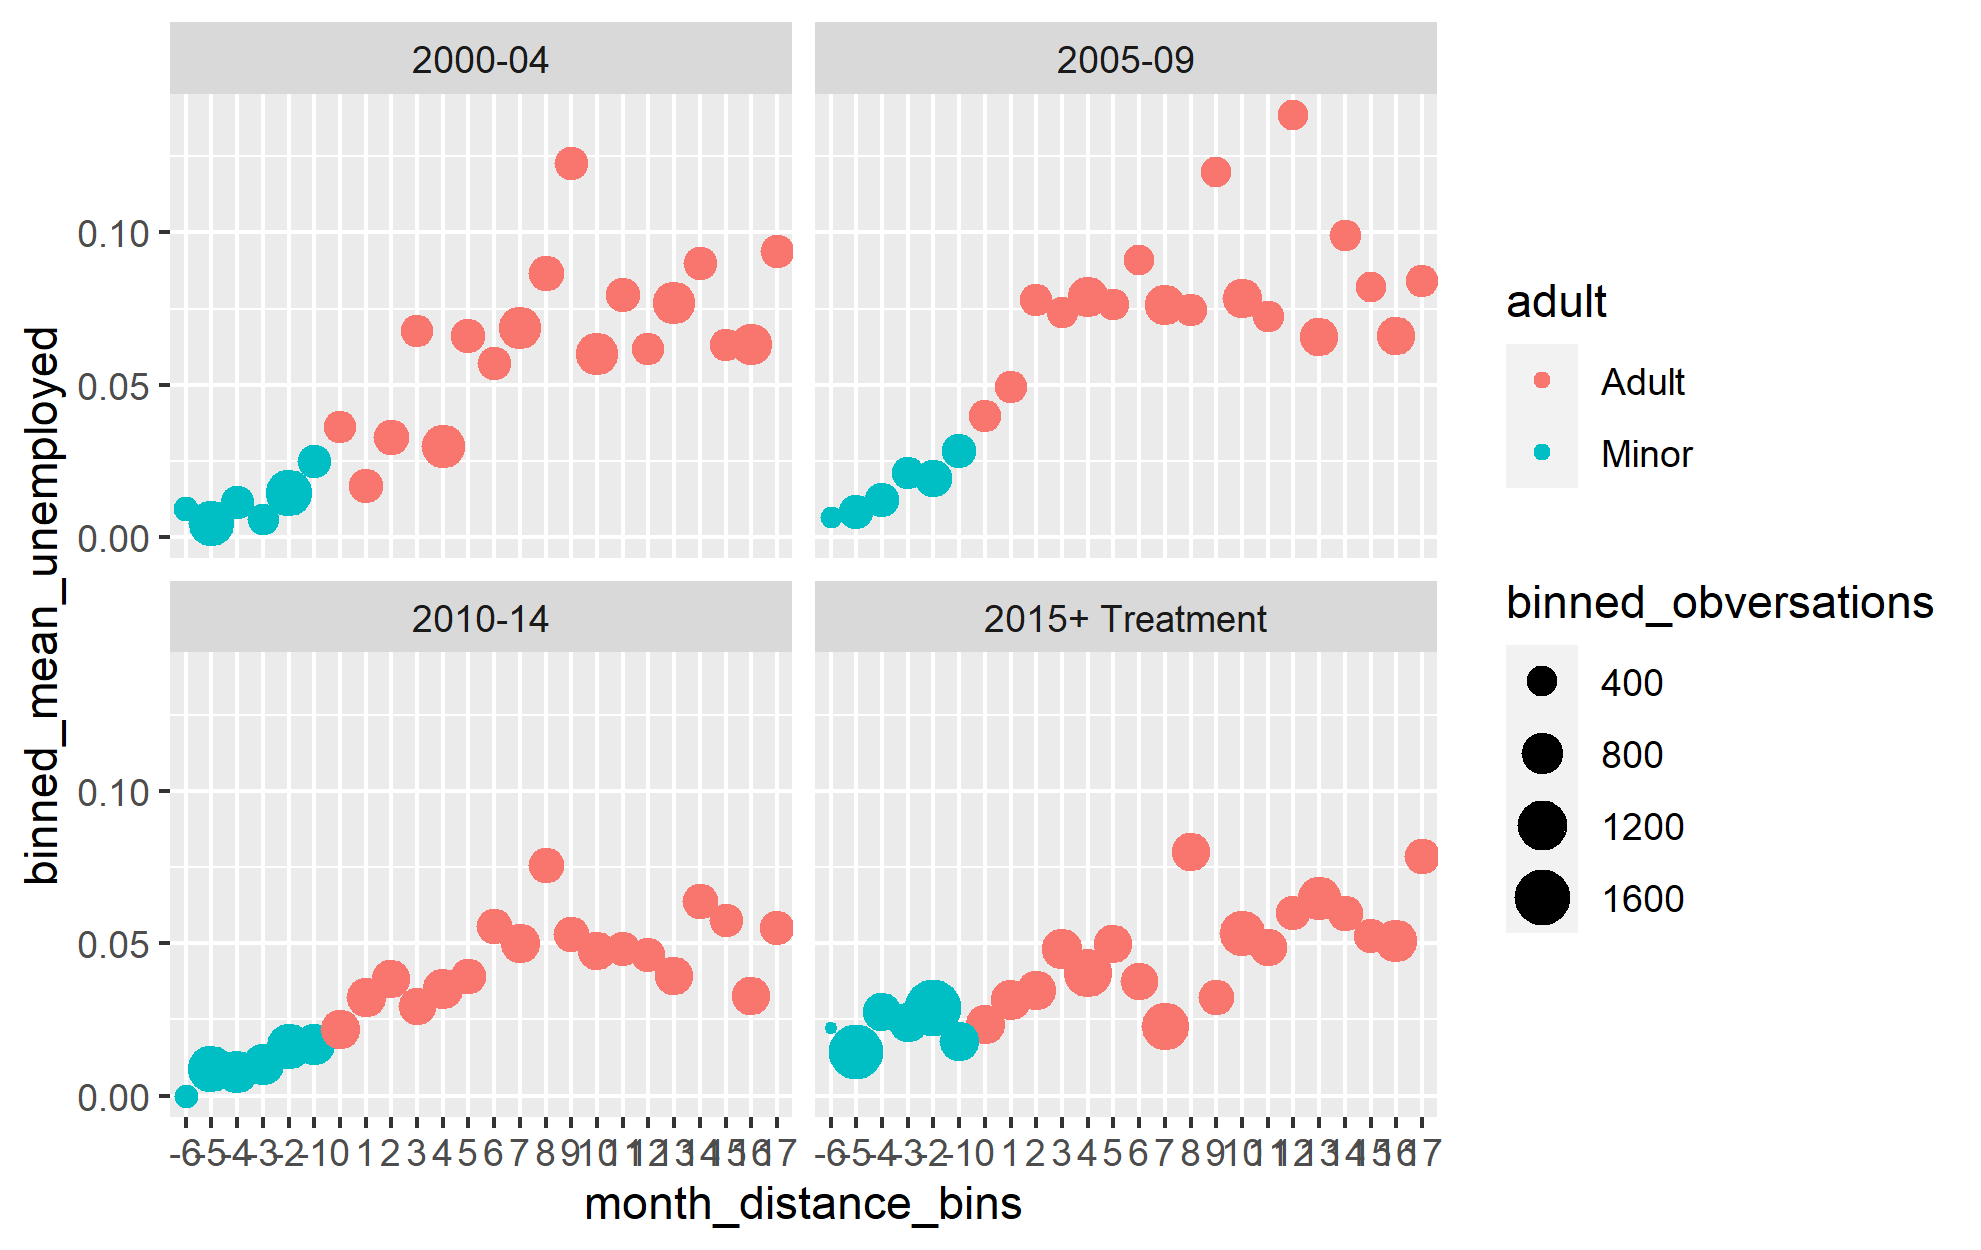
\includegraphics{../../plots/binned_unemp_scatter.png}}
	\end{figure}
\end{frame}

\begin{frame}
	\begin{figure}
		\centering
		\resizebox{\textwidth}{!}{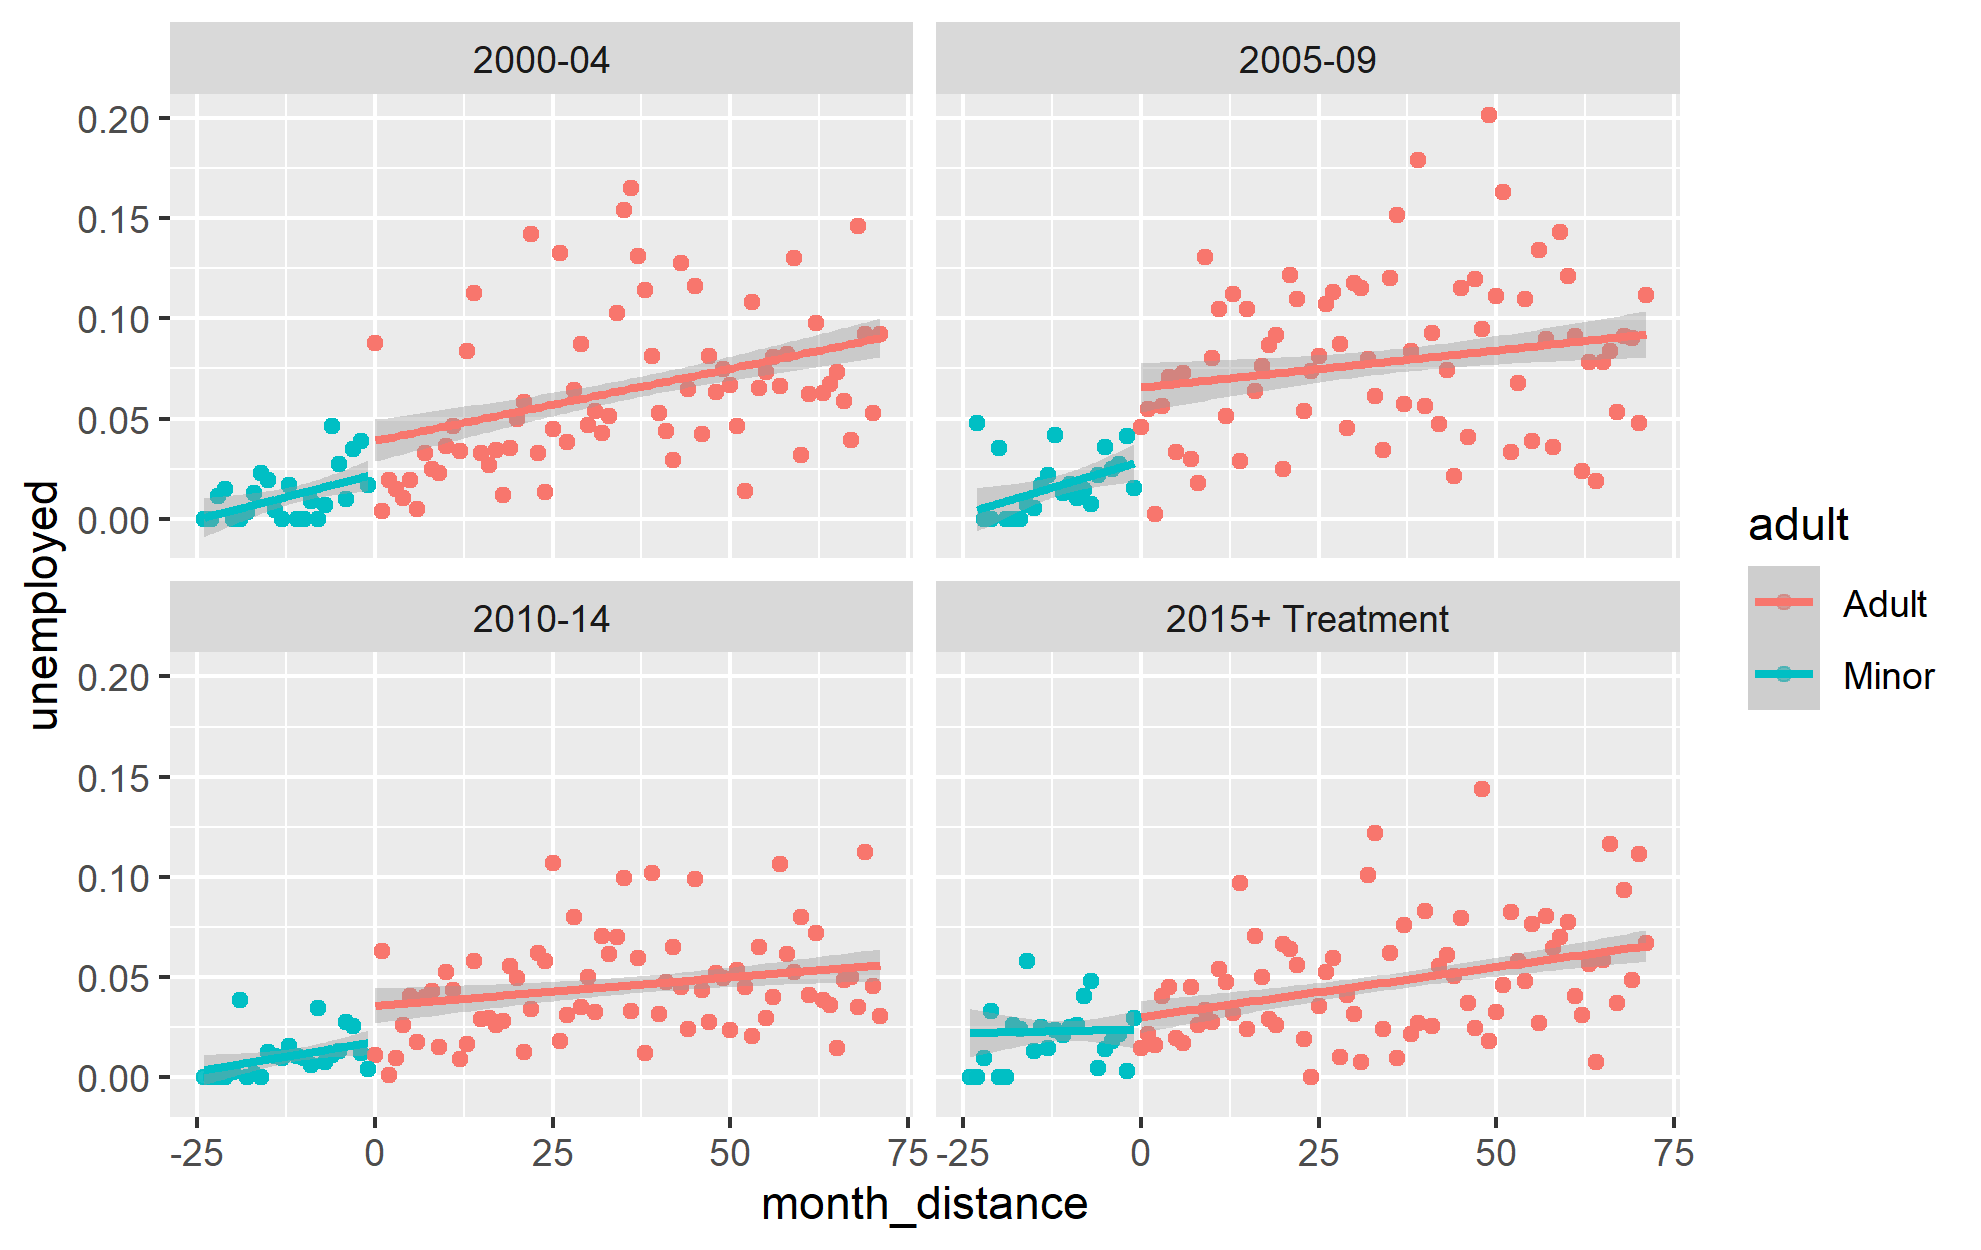
\includegraphics{../../plots/unemp_linear.png}}
	\end{figure}
\end{frame}

\begin{frame}
	\begin{figure}
		\centering
		\resizebox{\textwidth}{!}{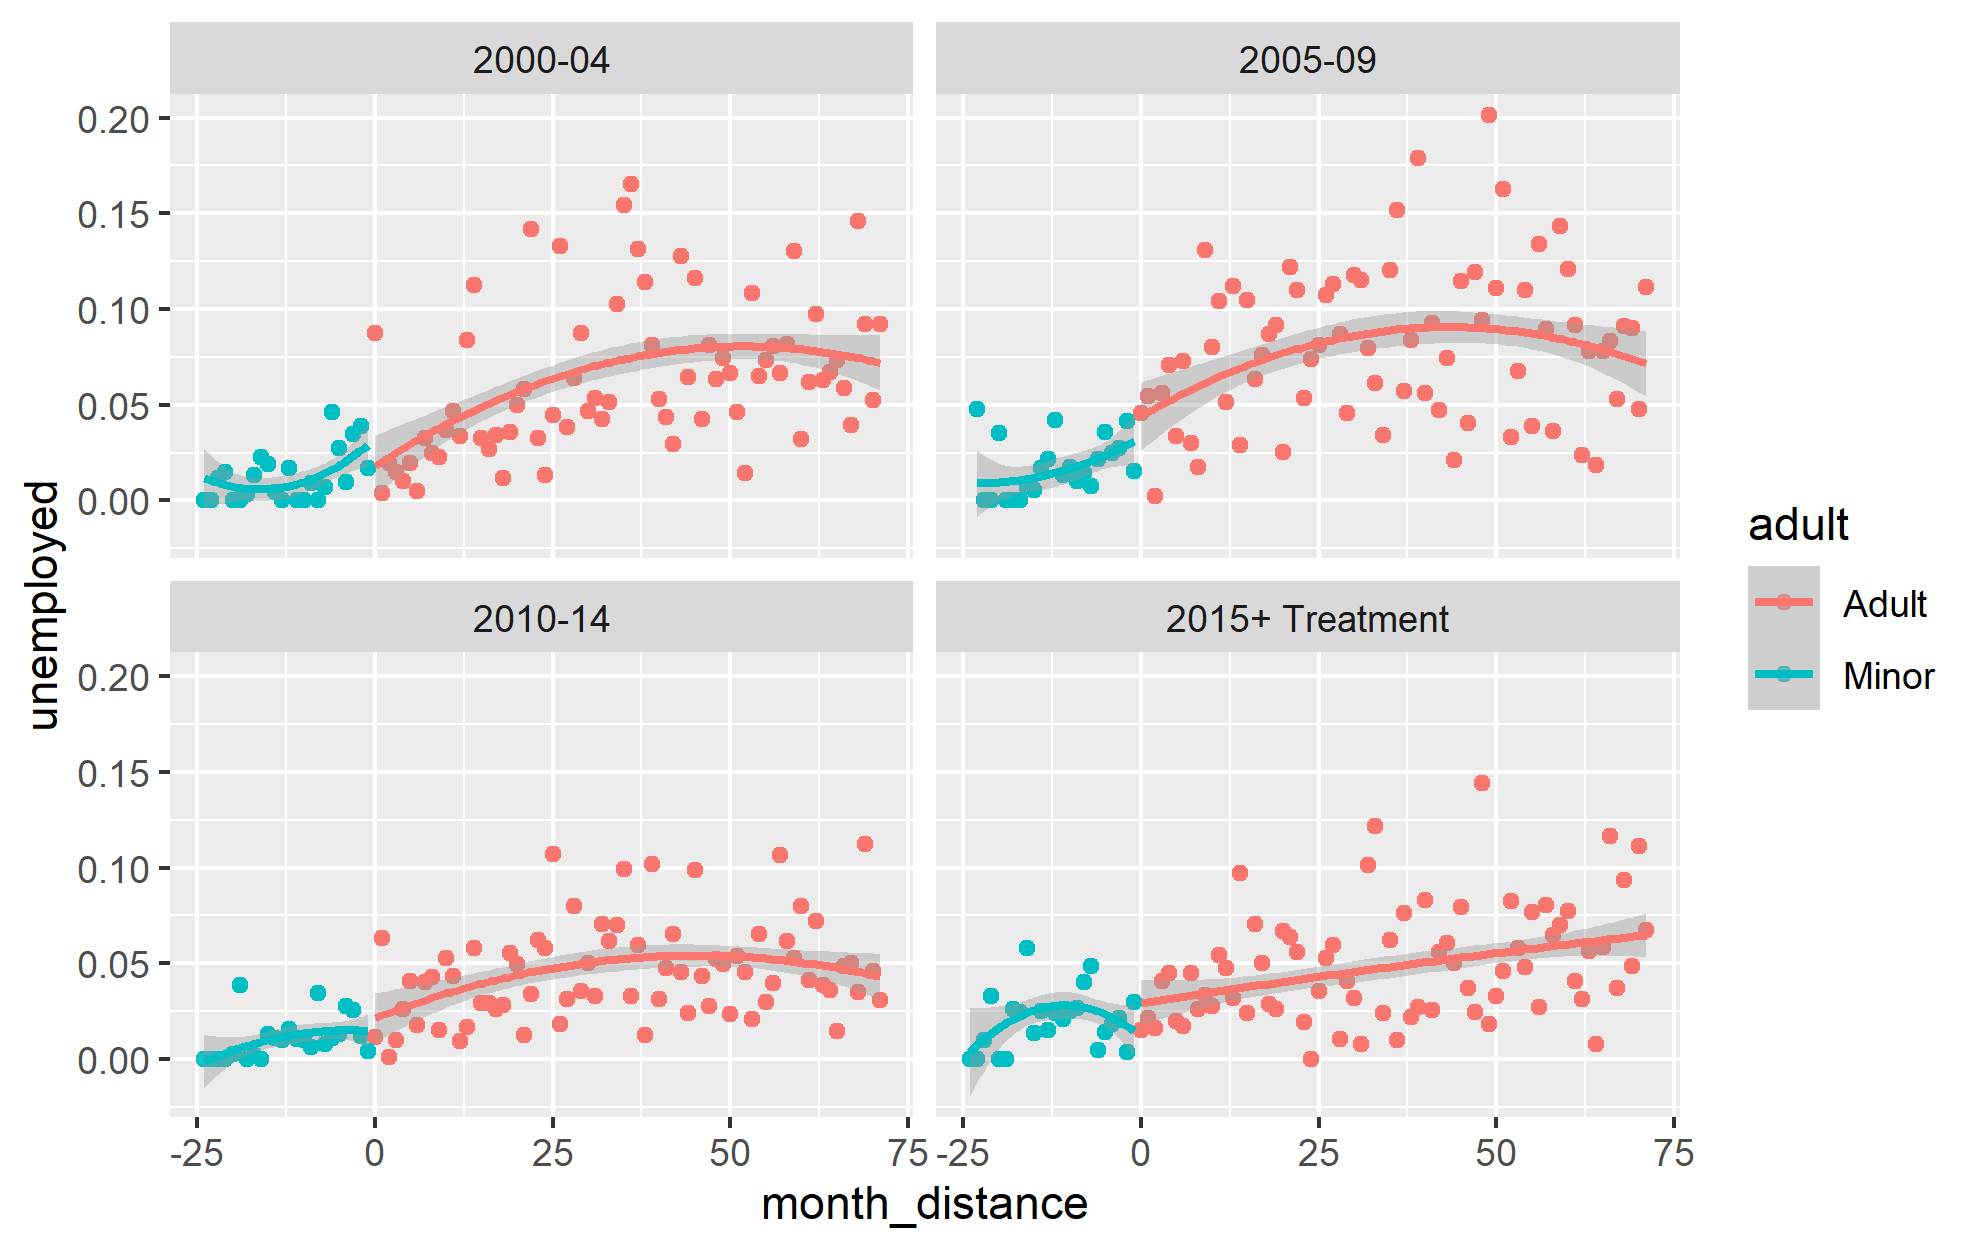
\includegraphics{../../plots/unemp_quadratic.png}}
	\end{figure}
\end{frame}



\begin{frame}
	\begin{figure}
		\centering
		\resizebox{\textwidth}{!}{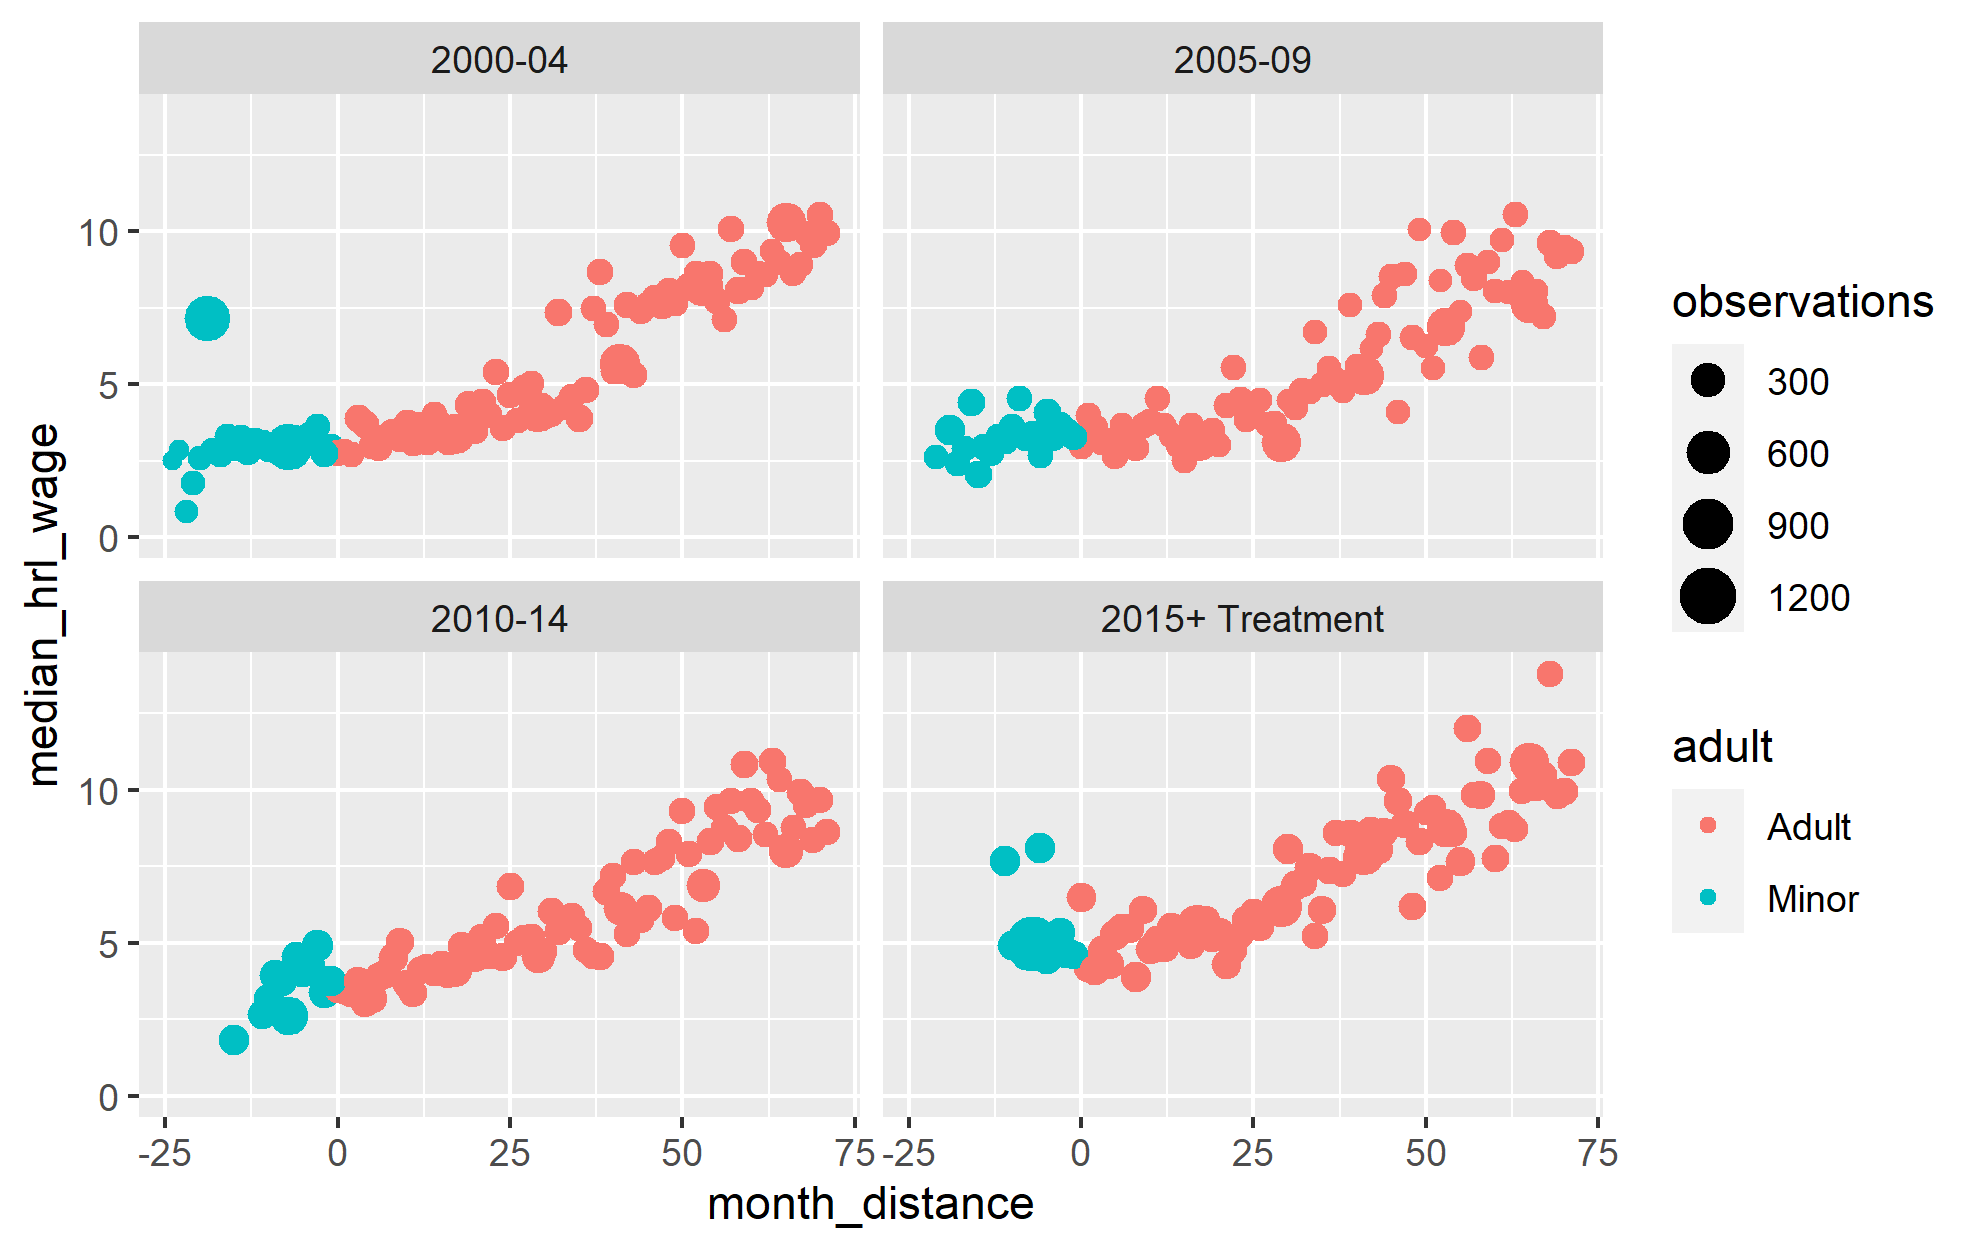
\includegraphics{../../plots/sbinned_hrl_wage_scatter.png}}
	\end{figure}
\end{frame}

\begin{frame}
	\begin{figure}
		\centering
		\resizebox{\textwidth}{!}{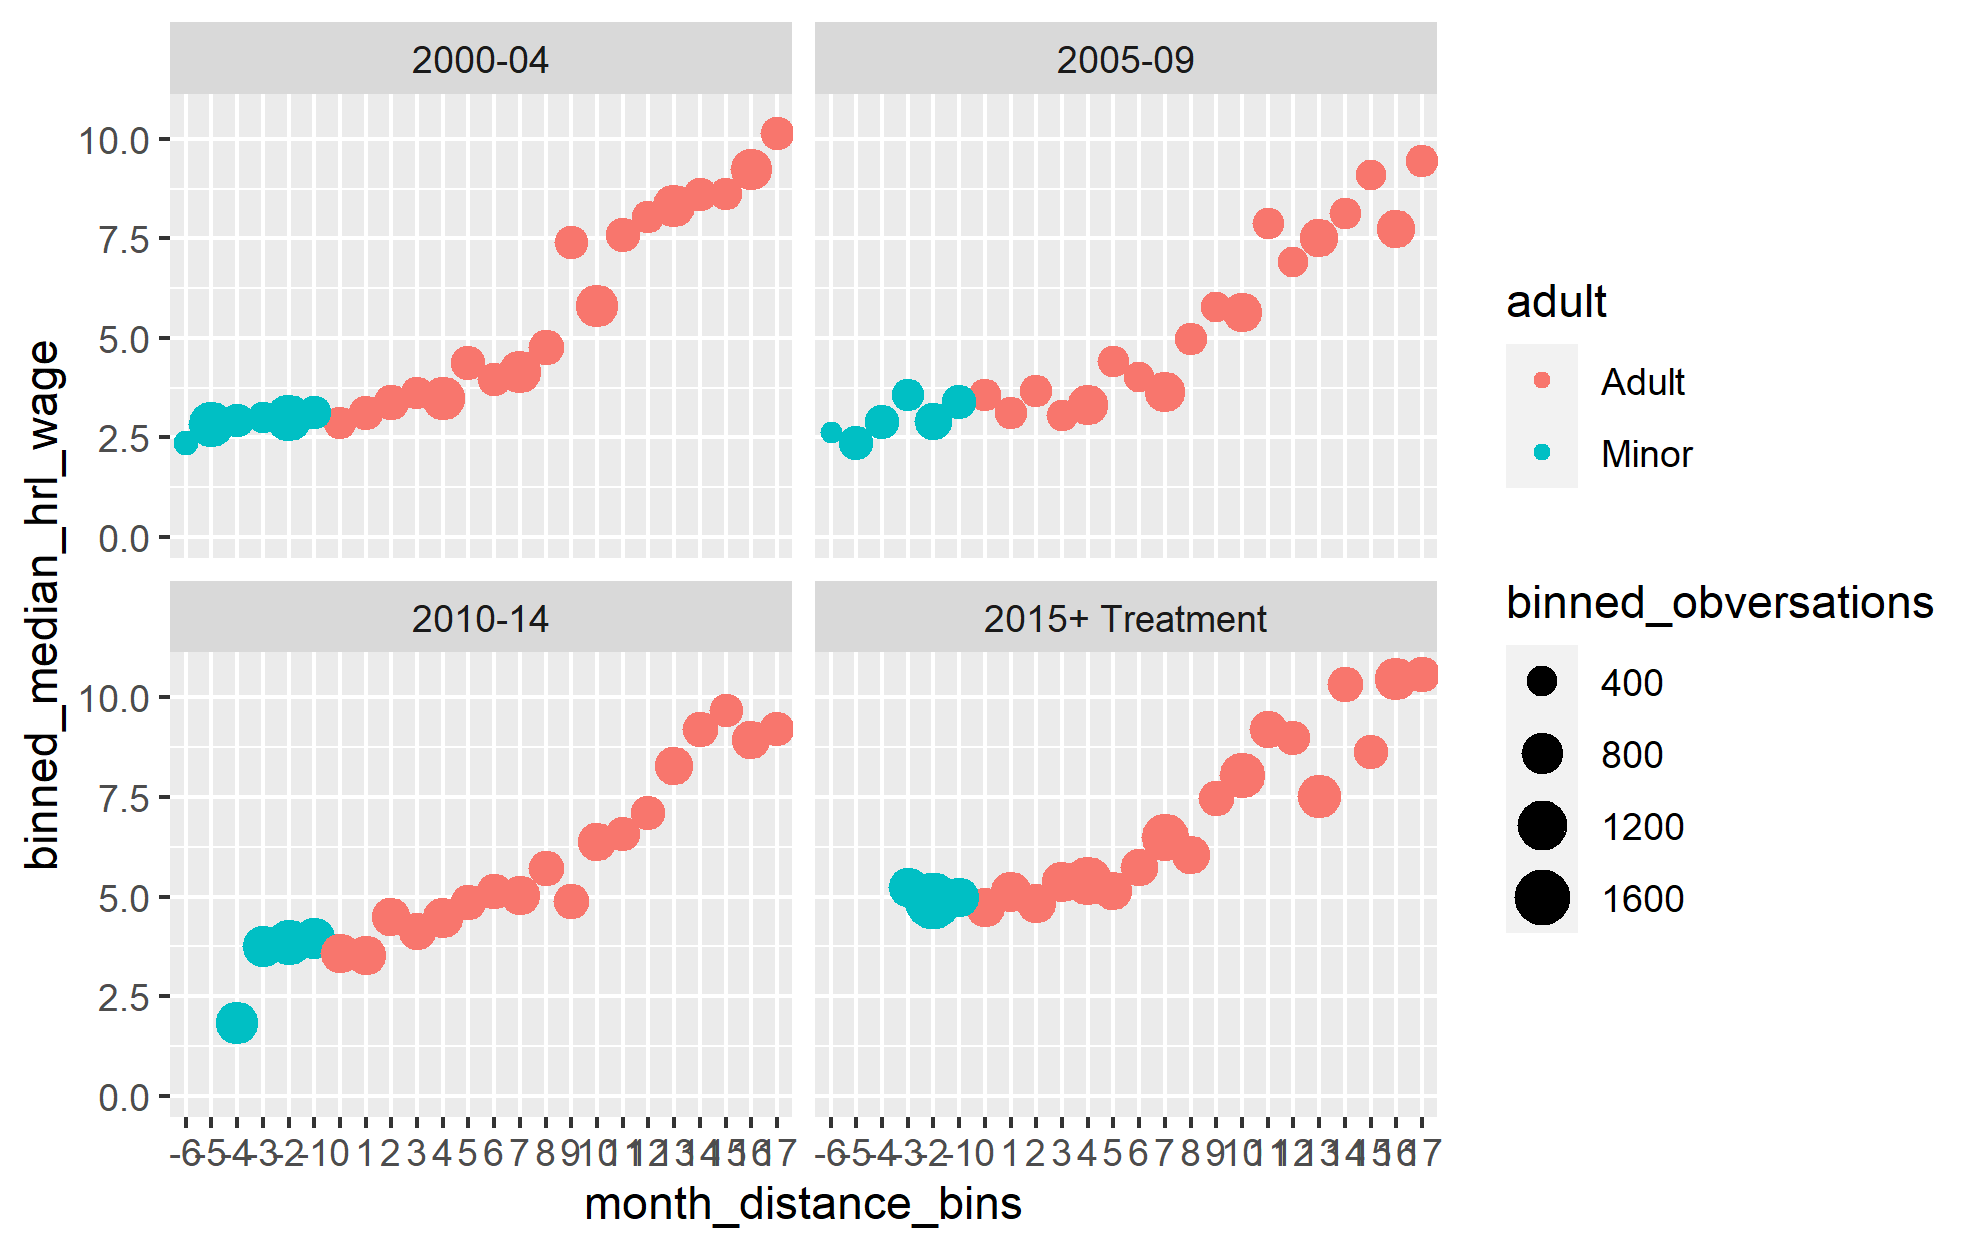
\includegraphics{../../plots/binned_hrl_wage_scatter.png}}
	\end{figure}
\end{frame}

\begin{frame}
	\begin{figure}
		\centering
		\resizebox{\textwidth}{!}{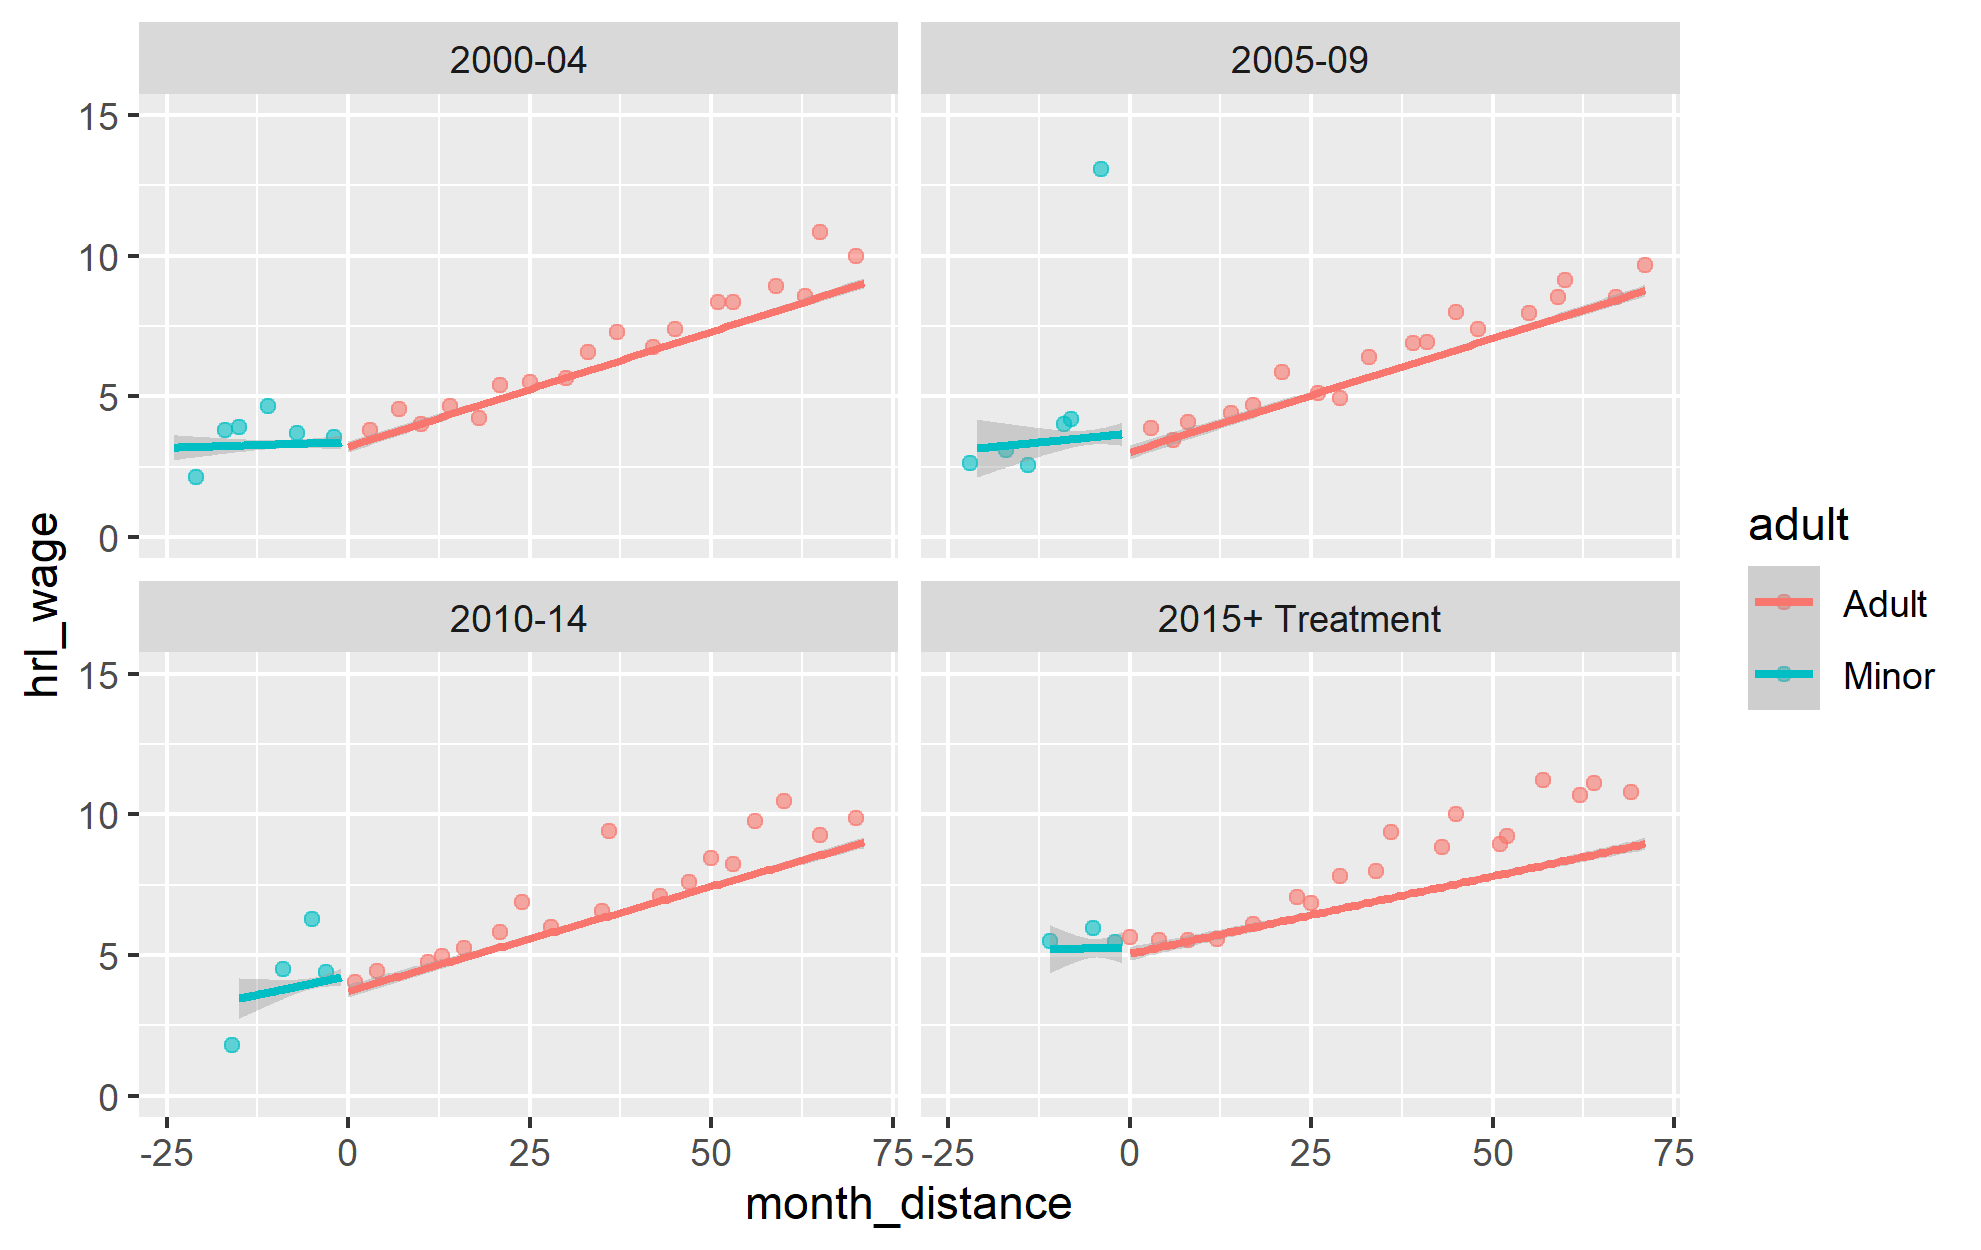
\includegraphics{../../plots/hrl_wage_linear.png}}
	\end{figure}
\end{frame}

\begin{frame}
	\begin{figure}
		\centering
		\resizebox{\textwidth}{!}{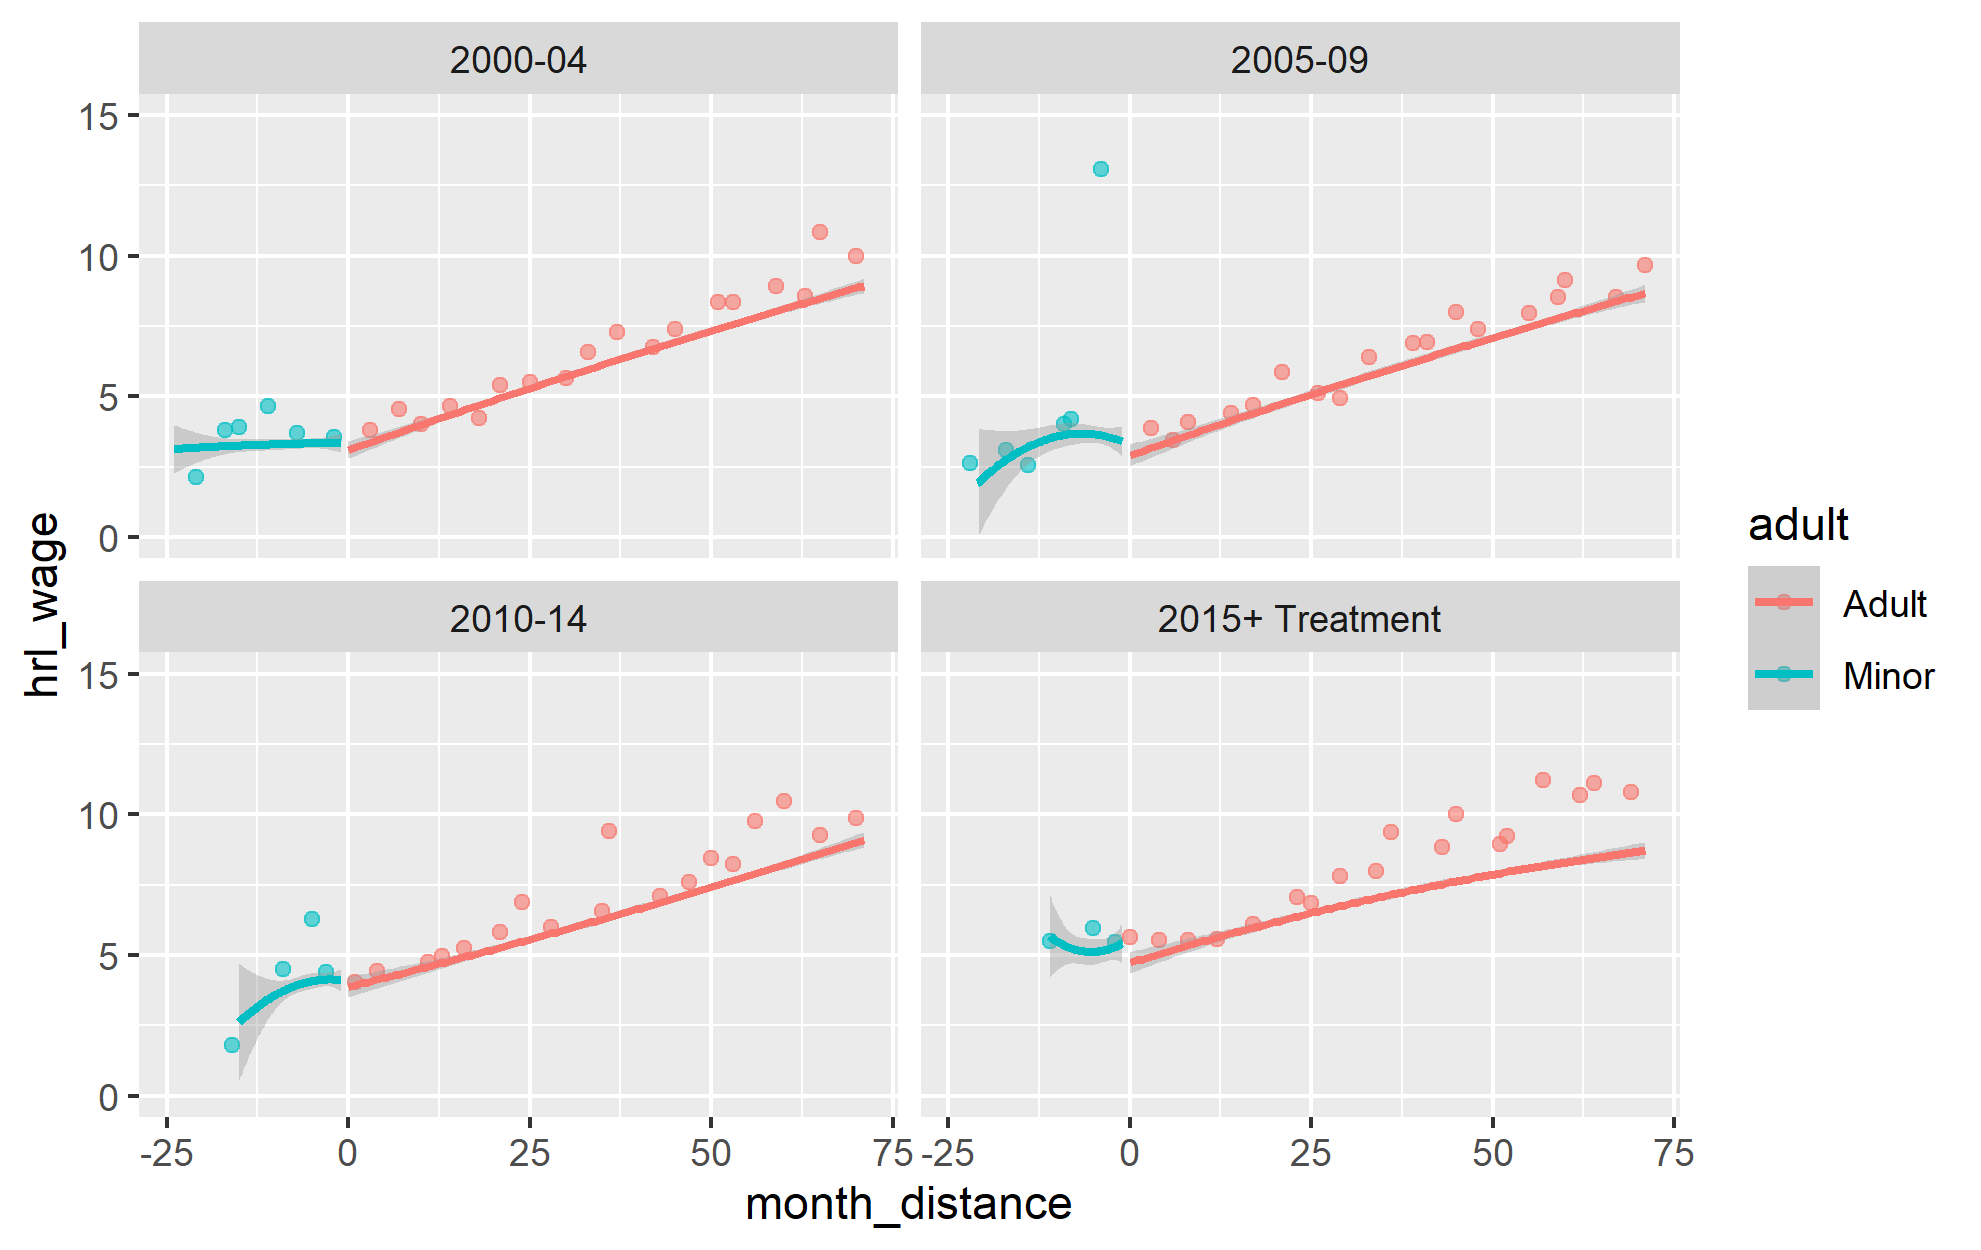
\includegraphics{../../plots/hrl_wage_quadratic.png}}
	\end{figure}
\end{frame}





\begin{frame}{Frame Title}
\begin{table}[!htbp] \centering 
	\caption{F-Test for R-squared} 
	\label{} 
	\begin{tabular}{@{\extracolsep{5pt}} ccc} 
		\\[-1.8ex]\hline 
		\hline \\[-1.8ex] 
		& F & Pr(\textgreater F) \\ 
		\hline \\[-1.8ex] 
		Linear Interaction Model & $5.892$ & $3.65e-17$ \\ 
		Quadratic Interaction Model & $5.880$ & $4.07e-17$ \\ 
		\hline \\[-1.8ex] 
	\end{tabular} 
\end{table} 
\end{frame}

\begin{frame}
	\begin{table}[!htbp] \centering 
		\caption{Global parametric spec on employment rate} 
		\label{} 
		\resizebox{1.04\textwidth}{!}{
		\begin{tabular}{@{\extracolsep{5pt}}lcccccc} 
			\\[-1.8ex]\hline 
			\hline \\[-1.8ex] 
			& \multicolumn{6}{c}{\textit{Dependent variable:}} \\ 
			\cline{2-7} 
			\\[-1.8ex] & \multicolumn{6}{c}{workforce} \\ 
			& linear interaction & linear interaction control & linear interaction covariates & linear interaction covariates control & quadratic interaction & quadratic interaction covariates \\ 
			\\[-1.8ex] & (1) & (2) & (3) & (4) & (5) & (6)\\ 
			\hline \\[-1.8ex] 
			month\_distance & 0.002 & $-$0.007$^{***}$ & 0.006$^{*}$ & $-$0.001 & $-$0.002 & 0.008 \\ 
			& (0.001) & (0.001) & (0.003) & (0.003) & (0.005) & (0.012) \\ 
			& & & & & & \\ 
			adult\_dummy & $-$0.047$^{***}$ & $-$0.004 & $-$0.017 & 0.023 & $-$0.059$^{**}$ & $-$0.073 \\ 
			& (0.018) & (0.018) & (0.034) & (0.036) & (0.029) & (0.054) \\ 
			& & & & & & \\ 
			dist\_x\_adult & 0.005$^{***}$ & 0.015$^{***}$ & 0.0004 & 0.008$^{**}$ & 0.011$^{**}$ & 0.003 \\ 
			& (0.001) & (0.001) & (0.003) & (0.003) & (0.005) & (0.012) \\ 
			& & & & & & \\ 
			migback &  &  & 0.009 & $-$0.019$^{***}$ &  & 0.009 \\ 
			&  &  & (0.006) & (0.007) &  & (0.006) \\ 
			& & & & & & \\ 
			pgbilzeit &  &  & 0.038$^{***}$ & 0.046$^{***}$ &  & 0.037$^{***}$ \\ 
			&  &  & (0.003) & (0.004) &  & (0.003) \\ 
			& & & & & & \\ 
			pgpsbil &  &  & $-$0.063$^{***}$ & $-$0.096$^{***}$ &  & $-$0.064$^{***}$ \\ 
			&  &  & (0.004) & (0.005) &  & (0.004) \\ 
			& & & & & & \\ 
			month\_distance\_sq &  &  &  &  & $-$0.0002 & 0.0001 \\ 
			&  &  &  &  & (0.0002) & (0.001) \\ 
			& & & & & & \\ 
			dist\_sq\_x\_adult &  &  &  &  & 0.0001 & $-$0.0001 \\ 
			&  &  &  &  & (0.0002) & (0.001) \\ 
			& & & & & & \\ 
			Constant & 0.164$^{***}$ & 0.073$^{***}$ & $-$0.100$^{**}$ & $-$0.183$^{***}$ & 0.149$^{***}$ & $-$0.089 \\ 
			& (0.016) & (0.016) & (0.043) & (0.048) & (0.026) & (0.058) \\ 
			& & & & & & \\ 
			\hline \\[-1.8ex] 
			Observations & 19,314 & 15,859 & 9,676 & 8,259 & 19,314 & 9,676 \\ 
			R$^{2}$ & 0.112 & 0.125 & 0.125 & 0.165 & 0.112 & 0.126 \\ 
			Adjusted R$^{2}$ & 0.111 & 0.125 & 0.124 & 0.164 & 0.112 & 0.126 \\ 
			Residual Std. Error & 17.481 (df = 15997) & 20.530 (df = 14135) & 18.294 (df = 9513) & 22.128 (df = 7986) & 17.477 (df = 15995) & 18.281 (df = 9511) \\ 
			F Statistic & 670.106$^{***}$ (df = 3; 15997) & 673.194$^{***}$ (df = 3; 14135) & 226.440$^{***}$ (df = 6; 9513) & 262.178$^{***}$ (df = 6; 7986) & 404.121$^{***}$ (df = 5; 15995) & 172.006$^{***}$ (df = 8; 9511) \\ 
			\hline 
			\hline \\[-1.8ex] 
			\textit{Note:}  & \multicolumn{6}{r}{$^{*}$p$<$0.1; $^{**}$p$<$0.05; $^{***}$p$<$0.01} \\ 
		\end{tabular} }
	\end{table} 
\end{frame}

\begin{frame}
	\begin{table}[!htbp] \centering 
		\vspace{-7mm}
		\caption{Global parametric spec on unemployment rate} 
		\label{} 
		\resizebox{1.04\textwidth}{!}{
		\begin{tabular}{@{\extracolsep{5pt}}lcccccc} 
			\\[-1.8ex]\hline 
			\hline \\[-1.8ex] 
			& \multicolumn{6}{c}{\textit{Dependent variable:}} \\ 
			\cline{2-7} 
			\\[-1.8ex] & \multicolumn{6}{c}{unemployed} \\ 
			& linear interaction & linear interaction control & linear interaction covariates & linear interaction covariates control & quadratic interaction & quadratic interaction covariates \\ 
			\\[-1.8ex] & (1) & (2) & (3) & (4) & (5) & (6)\\ 
			\hline \\[-1.8ex] 
			month\_distance & 0.0001 & 0.001 & $-$0.002 & 0.001 & $-$0.003 & 0.005 \\ 
			& (0.001) & (0.001) & (0.002) & (0.002) & (0.003) & (0.006) \\ 
			& & & & & & \\ 
			adult\_dummy & 0.006 & 0.018$^{**}$ & 0.033$^{**}$ & 0.039$^{**}$ & 0.018 & 0.005 \\ 
			& (0.008) & (0.008) & (0.016) & (0.017) & (0.014) & (0.025) \\ 
			& & & & & & \\ 
			dist\_x\_adult & 0.0004 & $-$0.0003 & 0.003 & $-$0.00000 & 0.004 & $-$0.004 \\ 
			& (0.001) & (0.001) & (0.002) & (0.002) & (0.003) & (0.006) \\ 
			& & & & & & \\ 
			migback &  &  & 0.003 & 0.001 &  & 0.003 \\ 
			&  &  & (0.003) & (0.003) &  & (0.003) \\ 
			& & & & & & \\ 
			pgbilzeit &  &  & $-$0.020$^{***}$ & $-$0.031$^{***}$ &  & $-$0.020$^{***}$ \\ 
			&  &  & (0.001) & (0.002) &  & (0.001) \\ 
			& & & & & & \\ 
			pgpsbil &  &  & $-$0.010$^{***}$ & 0.007$^{***}$ &  & $-$0.010$^{***}$ \\ 
			&  &  & (0.002) & (0.002) &  & (0.002) \\ 
			& & & & & & \\ 
			month\_distance\_sq &  &  &  &  & $-$0.0001 & 0.0004 \\ 
			&  &  &  &  & (0.0001) & (0.0003) \\ 
			& & & & & & \\ 
			dist\_sq\_x\_adult &  &  &  &  & 0.0001 & $-$0.0004 \\ 
			&  &  &  &  & (0.0001) & (0.0003) \\ 
			& & & & & & \\ 
			Constant & 0.024$^{***}$ & 0.018$^{**}$ & 0.244$^{***}$ & 0.314$^{***}$ & 0.012 & 0.268$^{***}$ \\ 
			& (0.008) & (0.007) & (0.020) & (0.023) & (0.012) & (0.027) \\ 
			& & & & & & \\ 
			\hline \\[-1.8ex] 
			Observations & 15,366 & 14,363 & 9,670 & 8,258 & 15,366 & 9,670 \\ 
			R$^{2}$ & 0.004 & 0.006 & 0.043 & 0.048 & 0.004 & 0.044 \\ 
			Adjusted R$^{2}$ & 0.004 & 0.006 & 0.043 & 0.047 & 0.004 & 0.043 \\ 
			Residual Std. Error & 8.210 (df = 15126) & 9.144 (df = 13941) & 8.641 (df = 9507) & 10.532 (df = 7985) & 8.210 (df = 15124) & 8.641 (df = 9505) \\ 
			F Statistic & 22.262$^{***}$ (df = 3; 15126) & 28.776$^{***}$ (df = 3; 13941) & 72.018$^{***}$ (df = 6; 9507) & 66.986$^{***}$ (df = 6; 7985) & 13.673$^{***}$ (df = 5; 15124) & 54.269$^{***}$ (df = 8; 9505) \\ 
			\hline 
			\hline \\[-1.8ex] 
			\textit{Note:}  & \multicolumn{6}{r}{$^{*}$p$<$0.1; $^{**}$p$<$0.05; $^{***}$p$<$0.01} \\ 
		\end{tabular} }
	\end{table}  
\end{frame}

\begin{frame}
\begin{table}[!htbp] \centering 
	\caption{Global parametric spec on hourly wage} 
	\label{} 
	\resizebox{1.04\textwidth}{!}{
	\begin{tabular}{@{\extracolsep{5pt}}lcccccc} 
		\\[-1.8ex]\hline 
		\hline \\[-1.8ex] 
		& \multicolumn{6}{c}{\textit{Dependent variable:}} \\ 
		\cline{2-7} 
		\\[-1.8ex] & \multicolumn{6}{c}{hrl\_wage} \\ 
		& linear interaction & linear interaction control & linear interaction covariates & linear interaction covariates control & quadratic interaction & quadratic interaction covariates \\ 
		\\[-1.8ex] & (1) & (2) & (3) & (4) & (5) & (6)\\ 
		\hline \\[-1.8ex] 
		month\_distance & $-$0.014 & 0.002 & $-$0.137 & 0.016 & $-$0.114 & $-$0.513 \\ 
		& (0.164) & (0.155) & (0.205) & (0.138) & (0.610) & (0.772) \\ 
		& & & & & & \\ 
		adult\_dummy & $-$0.739 & $-$1.045 & 0.115 & $-$1.814$^{**}$ & $-$0.845 & 0.532 \\ 
		& (0.895) & (0.885) & (1.164) & (0.777) & (1.434) & (1.881) \\ 
		& & & & & & \\ 
		dist\_x\_adult & 0.109 & 0.088 & 0.223 & 0.063 & 0.230 & 0.621 \\ 
		& (0.164) & (0.155) & (0.205) & (0.138) & (0.611) & (0.773) \\ 
		& & & & & & \\ 
		migback &  &  & 0.249$^{**}$ & $-$0.080 &  & 0.249$^{**}$ \\ 
		&  &  & (0.121) & (0.115) &  & (0.121) \\ 
		& & & & & & \\ 
		pgbilzeit &  &  & 0.659$^{***}$ & 0.938$^{***}$ &  & 0.656$^{***}$ \\ 
		&  &  & (0.062) & (0.063) &  & (0.062) \\ 
		& & & & & & \\ 
		pgpsbil &  &  & $-$0.951$^{***}$ & $-$1.105$^{***}$ &  & $-$0.953$^{***}$ \\ 
		&  &  & (0.090) & (0.086) &  & (0.090) \\ 
		& & & & & & \\ 
		month\_distance\_sq &  &  &  &  & $-$0.010 & $-$0.036 \\ 
		&  &  &  &  & (0.058) & (0.071) \\ 
		& & & & & & \\ 
		dist\_sq\_x\_adult &  &  &  &  & 0.009 & 0.036 \\ 
		&  &  &  &  & (0.058) & (0.071) \\ 
		& & & & & & \\ 
		Constant & 5.619$^{***}$ & 5.077$^{***}$ & $-$0.206 & $-$1.737$^{*}$ & 5.433$^{***}$ & $-$0.911 \\ 
		& (0.872) & (0.853) & (1.280) & (0.948) & (1.397) & (1.943) \\ 
		& & & & & & \\ 
		\hline \\[-1.8ex] 
		Observations & 4,898 & 4,984 & 3,754 & 3,973 & 4,898 & 3,754 \\ 
		R$^{2}$ & 0.091 & 0.063 & 0.127 & 0.176 & 0.091 & 0.127 \\ 
		Adjusted R$^{2}$ & 0.091 & 0.062 & 0.126 & 0.175 & 0.090 & 0.126 \\ 
		Residual Std. Error & 275.240 (df = 4790) & 356.240 (df = 4821) & 263.533 (df = 3667) & 260.526 (df = 3835) & 275.259 (df = 4788) & 263.554 (df = 3665) \\ 
		F Statistic & 160.015$^{***}$ (df = 3; 4790) & 107.748$^{***}$ (df = 3; 4821) & 88.984$^{***}$ (df = 6; 3667) & 136.859$^{***}$ (df = 6; 3835) & 96.260$^{***}$ (df = 5; 4788) & 66.906$^{***}$ (df = 8; 3665) \\ 
		\hline 
		\hline \\[-1.8ex] 
		\textit{Note:}  & \multicolumn{6}{r}{$^{*}$p$<$0.1; $^{**}$p$<$0.05; $^{***}$p$<$0.01} \\ 
	\end{tabular} }
\end{table} 
\end{frame}

\begin{frame}
	\begin{table}[!htbp] \centering 
		\caption{Local parametric linear spec} 
		\label{} 
		\resizebox{\textwidth}{!}{
		\begin{tabular}{@{\extracolsep{5pt}}lccc} 
			\\[-1.8ex]\hline 
			\hline \\[-1.8ex] 
			& \multicolumn{3}{c}{\textit{Dependent variable:}} \\ 
			\cline{2-4} 
			\\[-1.8ex] & workforce & unemployed & hrl\_wage \\ 
			\\[-1.8ex] & (1) & (2) & (3)\\ 
			\hline \\[-1.8ex] 
			month\_distance & 0.002 & 0.0001 & $-$0.014 \\ 
			& (0.001) & (0.001) & (0.164) \\ 
			& & & \\ 
			adult\_dummy & $-$0.047$^{***}$ & 0.006 & $-$0.739 \\ 
			& (0.018) & (0.008) & (0.895) \\ 
			& & & \\ 
			dist\_x\_adult & 0.005$^{***}$ & 0.0004 & 0.109 \\ 
			& (0.001) & (0.001) & (0.164) \\ 
			& & & \\ 
			Constant & 0.164$^{***}$ & 0.024$^{***}$ & 5.619$^{***}$ \\ 
			& (0.016) & (0.008) & (0.872) \\ 
			& & & \\ 
			\hline \\[-1.8ex] 
			Observations & 19,314 & 15,366 & 4,898 \\ 
			R$^{2}$ & 0.112 & 0.004 & 0.091 \\ 
			Adjusted R$^{2}$ & 0.111 & 0.004 & 0.091 \\ 
			Residual Std. Error & 17.481 (df = 15997) & 8.210 (df = 15126) & 275.240 (df = 4790) \\ 
			F Statistic & 670.106$^{***}$ (df = 3; 15997) & 22.262$^{***}$ (df = 3; 15126) & 160.015$^{***}$ (df = 3; 4790) \\ 
			\hline 
			\hline \\[-1.8ex] 
			\textit{Note:}  & \multicolumn{3}{r}{$^{*}$p$<$0.1; $^{**}$p$<$0.05; $^{***}$p$<$0.01} \\ 
		\end{tabular} }
	\end{table} 
\end{frame}

\begin{frame}
	\begin{table}[!htbp] \centering 
		\caption{robustness to trimming sample} 
		\label{}
		\resizebox{1.04\textwidth}{!}{
		\begin{tabular}{@{\extracolsep{5pt}}lcccccc} 
			\\[-1.8ex]\hline 
			\hline \\[-1.8ex] 
			& \multicolumn{6}{c}{\textit{Dependent variable:}} \\ 
			\cline{2-7} 
			\\[-1.8ex] & \multicolumn{2}{c}{workforce} & \multicolumn{2}{c}{unemployed} & \multicolumn{2}{c}{hrl\_wage} \\ 
			& excluding 10 &  excluding 20 &  excluding 10 &  excluding 20&excluding 10&excluding 20\\ 
			\\[-1.8ex] & (1) & (2) & (3) & (4) & (5) & (6)\\ 
			\hline \\[-1.8ex] 
			month\_distance & 0.006 & 0.011 & $-$0.002 & $-$0.004 & $-$0.114 & $-$0.114 \\ 
			& (0.007) & (0.010) & (0.003) & (0.005) & (0.606) & (0.540) \\ 
			& & & & & & \\ 
			adult\_dummy & $-$0.068$^{**}$ & $-$0.067$^{*}$ & 0.010 & 0.020 & $-$0.638 & $-$0.691 \\ 
			& (0.032) & (0.036) & (0.015) & (0.016) & (1.429) & (1.277) \\ 
			& & & & & & \\ 
			dist\_x\_adult & 0.002 & $-$0.005 & 0.003 & 0.005 & 0.209 & 0.214 \\ 
			& (0.007) & (0.010) & (0.003) & (0.005) & (0.606) & (0.540) \\ 
			& & & & & & \\ 
			month\_distance\_sq & 0.0004 & 0.001 & $-$0.0001 & $-$0.0003 & $-$0.010 & $-$0.010 \\ 
			& (0.0004) & (0.001) & (0.0002) & (0.0003) & (0.057) & (0.051) \\ 
			& & & & & & \\ 
			dist\_sq\_x\_adult & $-$0.0004 & $-$0.001 & 0.0001 & 0.0003 & 0.010 & 0.010 \\ 
			& (0.0004) & (0.001) & (0.0002) & (0.0003) & (0.057) & (0.051) \\ 
			& & & & & & \\ 
			Constant & 0.169$^{***}$ & 0.180$^{***}$ & 0.015 & 0.009 & 5.433$^{***}$ & 5.433$^{***}$ \\ 
			& (0.029) & (0.034) & (0.013) & (0.015) & (1.387) & (1.236) \\ 
			& & & & & & \\ 
			\hline \\[-1.8ex] 
			Observations & 16,612 & 15,282 & 14,067 & 12,740 & 4,435 & 4,048 \\ 
			R$^{2}$ & 0.096 & 0.089 & 0.003 & 0.003 & 0.083 & 0.085 \\ 
			Adjusted R$^{2}$ & 0.096 & 0.088 & 0.003 & 0.003 & 0.082 & 0.084 \\ 
			Residual Std. Error & 17.608 (df = 13905) & 17.275 (df = 12593) & 7.998 (df = 13843) & 7.914 (df = 12534) & 273.373 (df = 4334) & 243.566 (df = 3954) \\ 
			F Statistic & 296.011$^{***}$ (df = 5; 13905) & 244.716$^{***}$ (df = 5; 12593) & 8.506$^{***}$ (df = 5; 13843) & 8.653$^{***}$ (df = 5; 12534) & 78.884$^{***}$ (df = 5; 4334) & 73.894$^{***}$ (df = 5; 3954) \\ 
			\hline 
			\hline \\[-1.8ex] 
			\textit{Note:}  & \multicolumn{6}{r}{$^{*}$p$<$0.1; $^{**}$p$<$0.05; $^{***}$p$<$0.01} \\ 
	\end{tabular} }
	\end{table} 
\end{frame}


\end{document}
